\documentclass[UTF8,twoside]{ctexbook}
\usepackage{ctexcap,geometry,amsmath,fancyhdr,listings,tabularx,xcolor,graphicx,multirow,enumerate,amssymb,amscd,extarrows,mathrsfs,rotating,verbatim}
\geometry{left=3cm,right=3cm,top=3.5cm,bottom=3.5cm}
\pagestyle{fancy}
\fancyhf{}
\renewcommand{\chaptername}{第\chinese{chapter}章}
\renewcommand{\chaptermark}[1]{\markboth{\chaptername\  #1}{}}
\fancyhead[RE]{\leftmark}
\fancyhead[LO]{\rightmark}
\fancyhead[LE,RO]{\thepage}
\title{《泛函分析选讲》习题参考解答}
\author{吴瀚霖 hlwu.bnu@gmail.com}
\date{\today}
\newtheorem{exercise}{习题}[section]
\renewcommand{\exp}[1]{\text e^{#1}}
\newcommand{\h}{\mathscr}
\newcommand{\kx}{\mathbb}
\newcommand{\mycap}[2]{\mathop{\cap}\limits_{#1}^{#2}}
\newcommand{\mycup}[2]{\mathop{\cup}\limits_{#1}^{#2}}
\numberwithin{equation}{section}
\newcommand{\lx}{\mathscr L (\mathscr X)}
\newcommand{\xlim}[1]{\mathop{\lim}\limits_{#1}} %显示角色
\def\QEDopen{{\setlength{\fboxsep}{0pt}\setlength{\fboxrule}{0.2pt}\fbox{\rule[0pt]{0pt}{1.3ex}\rule[0pt]{1.3ex}{0pt}}}} %定义空心符
\def\QED{\QEDopen} %
\def\proof{\noindent{\bf 证明}: }
\def\endproof{\hspace*{\fill}~\QED\par\endtrivlist\unskip}
%\geometry{a4paper,left=2cm,right=2cm,top=2cm,bottom=2cm}
\newcommand{\upcite}[1]{\textsuperscript{\textsuperscript{\cite{#1}}}}
\newcommand{\HRule}{\rule{\linewidth}{0.5mm}}
\begin{document}
	\begin{titlepage}
		\begin{center}

			% Title
			\ \vspace{2cm}

			%\HRule \\[1cm]
			{ \Huge \bfseries 《泛函分析选讲》}\\[0.4em] \huge{习题参考解答} \\[0.4em]
			\HRule \\[2cm]

			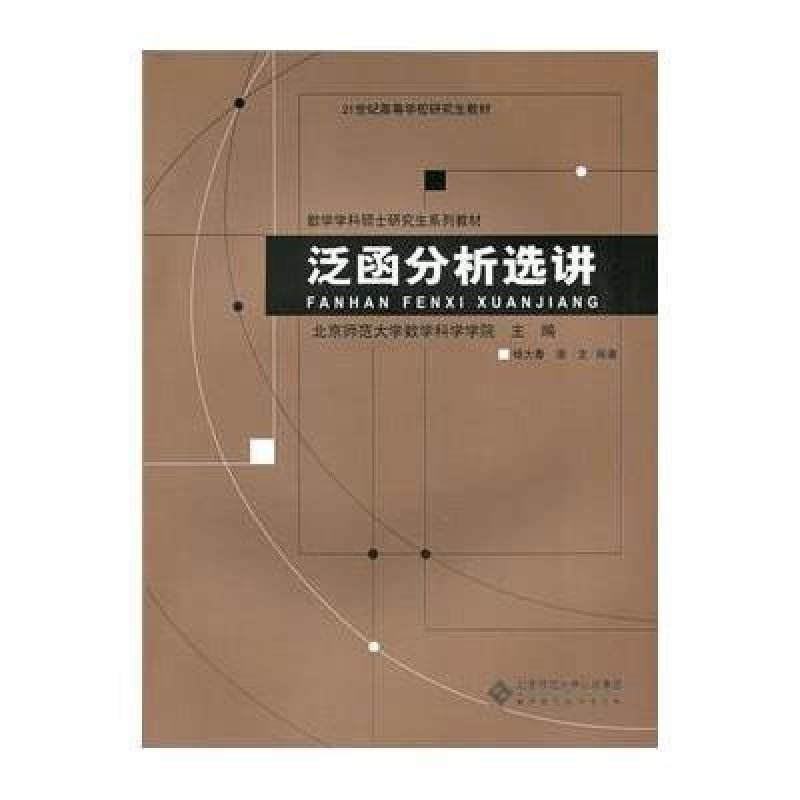
\includegraphics[width=0.4\textwidth]{pics/fm.jpg}
			% Author and supervisor

			\vfill

			% Bottom of the page
			{\large 吴瀚霖 \\ hlwu.bnu@gmail.com\\ \today}
		\end{center}
	\end{titlepage}
	\tableofcontents
	\chapter{紧算子的谱理论}
	\section{有界线性算子的谱}
	\begin{exercise}
		设$\h X$是一个有限维Banach空间,$A: \h X \rightarrow \h X$为有界线性算子. 则对于任意$\lambda \in \mathbb C$, $\lambda$必为$A$的正则值或特征值之一.
	\end{exercise}
	\begin{proof}
		若$A$为有限维空间$\h X$上的有界算子, 则$A$可由矩阵$(a_{ij})$表示. $A$单射当且仅当$A$满射. 从而$\lambda I-A $可逆当且仅当$\lambda E-A$可逆. 而当
		\begin{itemize}
			\item $\text{det}(\lambda E-A)=0$ 时, $\lambda\in\sigma(A)$;
			\item $\text{det}(\lambda E-A)\neq0$ 时, $\lambda\in\rho(A)$.
		\end{itemize}
		故对$\forall\lambda\in\mathbb C$, $\lambda$ 必为$A$的正则值或特征值.
	\end{proof}
	\begin{exercise}
		设$\h X$为一个 Banach 空间. 证明$\h L(\h X)$中的可逆(有有界逆)算子集为开集.
	\end{exercise}
	\begin{proof}
		$\forall A \in \h L(\h X)$ 且 $A^{-1}\in\h L(\h X)$. $\forall T\in \h L(\h X)$ 且 $\| T-A\|_{\lx}<\frac{1}{\|A^{-1}\|}$.
		\begin{align*}
		\| T^{-1}\| &= \| (T-A+A)^{-1} \| \\
		&=\| A^{-1}(I+(T-A)A^{-1})^{-1}  \| \\
		&\leq \| A^{-1} \|\cdot \|(I + (T-A)A^{-1})^{-1}\| \\
		&<\infty.
		\end{align*}
		由引理1.1.9, $\| (T-A)A^{-1} \|\leq \| T-A \|\cdot \| A^{-1} \|<1.$ 故$\lx$中的可逆算子为开集.
	\end{proof}

	\begin{exercise}
		考虑$\ell^2$上的左推移算子
		\[
		A: (\xi_1,\xi_2,\cdots)\mapsto(\xi_2,\xi_3,\cdots),
		\]
		证明$\sigma_p(A)=\{\lambda\in\mathbb C:|\lambda|<1\},\sigma_c(A)=\{\lambda\in\mathbb C:|\lambda|=1\}$且$\sigma_r(A)=\varnothing$.
	\end{exercise}
	\begin{proof}
		首先说明$A$是有界线性算子且$\|A\|=1$. 设
		\begin{align*}
		x&=(x_1,x_2,\cdots,x_n,\cdots)\in\ell^2, \\
		y&=Ax=(x_2,x_3,\cdots,x_{n+1},\cdots).
		\end{align*}
		有
		\[
		\|Ax\|^2=\sum_{n=2}^{\infty}|x_n|^2\leq\sum_{n=1}^{\infty}|x_n|^2=\|x\|^2
		\Longrightarrow
		\|Ax\|\leq\|x\|
		\Longrightarrow
		\|A\|\leq1.
		\]
		另一方面, $x':=(0,1,0\cdots)$, 则$Ax'=(1,0,0,\cdots)$, $\|Ax'\|=\|x'\|$. 故 $\|A\|=\sup\limits_{x\neq\theta}\frac{\|Ax\|}{\|x\|}=1.$

		(1) 当$|\lambda|>1$时, $|\lambda|>\|A\|\Longrightarrow \lambda\in\rho(A)$.

		(2) $D:=\{\lambda\in\kx C: |\lambda|<1\}.$ $\forall\lambda\in D, \{\lambda^n\}_{n=0}^\infty\in\ell^2.$ 因为
		\[
		A(1,\lambda,\lambda^2,\cdots)=(\lambda,\lambda^2,\cdots)=\lambda(1,\lambda,\lambda^2,\cdots),
		\]
		所以$\lambda\in\sigma_p(A).$

		(3) 先考虑$\lambda=1$时. 首先证明$(I-A)^{-1}$存在. $\forall x\in\ell^2$, 若$ (I-A)x=0$, 则
		\[
		(x_1,x_2,\cdots)=(x_2,x_3,\cdots).
		\]
		于是 $x=x_1(1,1,\cdots)$. 又因为$x\in\ell^2$, 所以$x_1=0$, 从而$x=\theta$. 即$(I-A)^{-1}$存在.

		下证$R(I-A)\neq\ell^2$, 但$\overline{R(I-A)}=\ell^2.$

		若$y=(I-A)x$, 则$y_k=x_k-x_{k+1}$, 即
		\[
		\left.
		\begin{aligned}
		y_1&=x_1-x_2\\
		y_2&=x_2-x_3\\
		&\cdots\\
		y_k&=x_k-x_{k+1}
		\end{aligned}
		\right\}
		\Longrightarrow
		\sum_{j=1}^k y_j=x_1-x_{k+1}.
		\]
		即$x_{k+1}=x_1-\sum_{j=1}^k y_j$. 易知, 非零分量为有限个的$y\in R(I-A)$. 事实上, 设$y$的非零分量个数为$K$, 取$x_1=\sum_{j=1}^k y_j$,
		\[
		x_{k+1}=\left\{
		\begin{aligned}
		&x_1-\sum_{j=1}^k y_j,k=1,2,\cdots,K\\
		&0,k>K
		\end{aligned}.
		\right.
		\]
		由上式可知, $x\in\ell^2$.

		存在$y\in\ell^2$, 但是$y\notin R(I-A)$. 事实上, 取$y=\{\frac{1}{j}\}_{j=1}^\infty\in\ell^2.$ 则
		\[
		x_{k+1}=x_1-\sum_{j=1}^{k}\frac{1}{j}\rightarrow -\infty,\ k\rightarrow\infty.
		\]
		所以, $x\notin\ell^2$, 也就是说$y\notin R(I-A)$, 那么$R(I-A)\neq\ell^2.$

		下证$\overline{R(I-A)}=\ell^2$, 为此, 设$\xi:=\{\xi_k\}_{k\in\kx N}$, $\forall\varepsilon\in(0,\infty)$. 存在$N\in\kx N$, 使得$\sum_{k=N+1}^\infty|\xi_k|^2<\varepsilon$. 令
		$y:=\{y_j\}_{j\in\kx N}$. 其中
		\[
		y_j=\left\{
		\begin{aligned}
		&\xi_j,j\leq  N\\
		&0,j>N.
		\end{aligned}
		\right.
		\]
		有
		\[
		\|y-\xi\|_{\ell^2}=\|\{\xi_j-y_j\}_{j=N+1}^{\infty}\|_{\ell^2}=\sum_{k=N+1}^\infty|\xi_k|^2<\varepsilon.
		\]
		故$\overline{R(I-A)}=\ell^2$. 从而$1\in\sigma_c(A)$.

		其次, 对于一般的$\lambda$使$|\lambda|=1$. 可以划归为$\lambda=1$ 的情形. 事实上,
		\[
		(\lambda I-A)x=y\Longleftrightarrow\lambda x_k-x_{k+1}=y_k\Longleftrightarrow\frac{x_k}{\lambda^k}-\frac{x_{k+1}}{\lambda^{k+1}}=\frac{y_k}{\lambda^{k+1}}, k=1,2,\cdots
		\]
		令$\xi_k=\frac{x_k}{\lambda^k},\eta_k=\frac{y_k}{\lambda^{k+1}},k=1,2,\cdots$. 则有$\xi_k-\xi_{k+1}=\eta_k,k=1,2,\cdots$. 即划归为$\lambda=1$ 的情形.
	\end{proof}

	\begin{exercise}
		考虑$L^2(0,+\infty)$上的微分算子:
		\[
		A:x(t)\mapsto x'(t).D(A)=H^1(0,+\infty).
		\]
		证明$\sigma_p(A)=\{\lambda\in\kx C:Re\lambda<0\}$. $\sigma_c(A)=\{\lambda\in\kx C:Re\lambda=0\}$且$\sigma_r(A)=\varnothing$. 其中$Re\lambda$表示$\lambda$ 的实部.
	\end{exercise}
	\begin{proof}
		记$\Omega:=(0,\infty)$. 由Meyers-Serrin定理有
		\[
		H^1(\Omega)=\{u\in L^2(\Omega):\widetilde{d}^\alpha u\in L^2(\Omega),|\alpha|=1\}.
		\]
		其中$\langle \widetilde{d}u,\varphi\rangle =(-1)^{|\alpha|}\langle u,\widetilde{d}^\alpha\varphi\rangle $. $\forall\varphi\in C_c^\infty(\Omega)$.

		先证明$A$是闭算子. 只需证明当$\{u_n\}_{n\in\kx N}\subset D(A)$. 且
		\[\left\{
		\begin{aligned}
		u_n\rightarrow u\ \text{in}\ L^2(\Omega)\\
		u_n'\rightarrow v\ \text{in}\ L^2(\Omega)
		\end{aligned} \right.\ \  (n\rightarrow\infty).
		\]
		时, 有$u\in D(A)$, 且$u'=v$. $\forall\varphi\in C_c^\infty(\Omega),\langle u_n',\varphi\rangle =-\langle u_n,\varphi'\rangle $. 从而由
		\[
		|\langle u_n,\varphi'\rangle -\langle u,\varphi'\rangle |=|\langle u_n-u,\varphi'\rangle |\leq\|u_n-u\|_{L^2(\Omega)}\|\varphi'\|_{L^2(\Omega)}\rightarrow0. (n\rightarrow\infty).
		\]
		知$\langle u_n',\varphi\rangle =-\langle u_n,\varphi'\rangle \rightarrow-\langle u,\varphi'\rangle $.

		类似可以证明$\langle u_n',\varphi\rangle\rightarrow\langle v,\varphi\rangle ,n\rightarrow\infty$. 即$\langle v,\varphi\rangle =-\langle u,\varphi'\rangle ,\forall\varphi\in C_c^\infty(\Omega)$ 成立. 由弱导数的定义知$u'=v\in L^2(\Omega)$. 从而$u\in H^1(\Omega)$, 且$u'=v$. 故$A$ 为闭算子.

		再证$\sigma_p(A)=\{\lambda\in\kx C:Re\lambda>0\}$. 考虑方程$(\lambda I-A)u=0$, 即$u'-\lambda u=0$. 由PDE知系数光滑从而弱解也光滑. 解ODE, $u'-\lambda u=0$. 得$u=0$ 或$ce^{\lambda x}\in L^2(\Omega)$. 故$(\lambda I-A)^{-1}$ 不存在. $\lambda\in\sigma_p(A)$.

		再证$\sigma_c(A)=\{\lambda\in\kx C:Re\lambda=0\}$. 先说明$R(\lambda I-A)\subsetneqq L^2(\Omega)$. 令$v(x):=\frac{e^{\lambda x}}{x+1}\in L^2(\Omega)$. 由$(\lambda I-A)u=v$得
		\[
		\begin{aligned}
		u(x)&=e^{\lambda x}[u(0)-\int_0^x e^{-\lambda t}v(t)dt]\\
		&=e^{\lambda x}[u(0)-\ln(x+1)]\notin L^2(\Omega).
		\end{aligned}
		\]
		故$R(\lambda I-A)\subsetneqq L^2(\Omega)$.

		再证$\overline{R(\lambda I-A)}=L^2(\Omega)$. 因$C_c^\infty(\Omega)=L^2(\Omega)$, 故只需说明$R(\lambda I-A)\supset C_c^\infty(\Omega)$. 事实上, 对$\forall v\in C_c^\infty(\Omega)$. $\exists M_v$, 使得$\text{supp}v\subset(0,M_v)$. 由$(\lambda I-A)u=v$, 得$u(x)=e^{\lambda x}[u(0)-\int_0^x e^{-\lambda x}v(t)dt]$. 令
		$u(0):=\int_0^{M_v}e^{-\lambda t}v(t)dt$. 则
		\[
		u(x)=\left\{
		\begin{aligned}
		&e^{\lambda x}\int_x^{M_v}e^{-\lambda x}v(t)dt,&x\in(0,M_v)\\
		&0,&x\in(M_v,\infty).
		\end{aligned}
		\right.
		\]
		满足$u\in H^1(\Omega)$. 即$R(\lambda I-A)\supset C_c^\infty(\Omega)$. 故$\overline{\lambda I-A}=L^2(\Omega)$.

		最后说明$\rho(A)\supset\{\lambda\in\kx C: Re\lambda>0\}$. 设$Re\lambda>0$, 此时$ce^{\lambda x}\notin L^2(\Omega)$. 从而$(\lambda I-A)^{-1}$存在. 断言$R(\lambda I-A)=L^2(\Omega)$. 事实上, 对$\forall v\in L^2(\Omega)$. 令$u(x)=e^{\lambda x}\int_0^\infty e^{\lambda t}v(t)dt=\int_0^\infty e^{-\lambda s}v(s+x)ds$. 则$u$ 满足$u'-\lambda u=v$ 且$u\in H^1(\Omega)$. 由Minkovski不等式, 有
		\[
		\begin{aligned}
		\|u\|_{L^2(\Omega)}&=\left\|\int_0^\infty e^{-\lambda x}v(s+x)ds\right\|_{L^2(\Omega)}\\
		&=\int_0^\infty|e^{-\lambda s}|ds\|v\|_{L^2(\Omega)}\\
		&=\frac{1}{Re\lambda}\|v\|_{L^2(\Omega)}\\
		&<\infty.
		\end{aligned}
		\]
		即$R(\lambda I-A)=L^2(\Omega)$. 由命题1.1.4知, $\lambda\in\rho(A)$. 故$\rho(A)=\{\lambda\in\kx C:Re\lambda>0\}$. 又因$\rho(A)\cup\sigma_p(A)\cup\sigma_c(A)\cup\sigma_r(A)=\kx C$ 且互不相交, 故结论得证.
	\end{proof}
	\begin{exercise}
		\begin{enumerate}[(1)]
			\item 证明(1.1.1)和(1.1.2)成立
			\item 利用$S^ny=\sum_{k=0}^{n}A^ky$给出引理1.1.9的另一个证明.
			\item $\forall x\in \kx R$, 定义$\kx R$上的线性算子$A_x:y\mapsto xy,\forall y\in\kx R$. 利用此算子说明当$|x|<1$时.
			\[
			(1-x)^{-1}=\sum_{k=0}^{\infty}x^k
			\]
			只是(1.1.3)的一个特例.
		\end{enumerate}
	\end{exercise}
	\begin{proof}
		(1)因为$\|\sum_{n=0}^{N}A^n\|_{\h L(\h X)}\leq\sum_{n=0}^{N}\|A^n\|_{\h L(\h X)}\leq\sum_{n=0}^{N}\|A\|^n_{\h L(\h X)}$. 所以$\forall k,N\in\kx N$,
		\[
		\|\sum_{n=N}^{N+k}A^n\|_{\h L(\h X)}\leq\sum_{n=N}^{N+k}\|A\|^n_{\h L(\h X)}\xrightarrow{\|A\|_{\h L(\h X)}<1} 0, N\rightarrow\infty.
		\]
		故$\{\sum_{n=0}^{N}A^n\}_{N\in\kx N}$为$\h L(\h X)$中的基本列. 而$\h L(\h X)$ 为Banach空间, 故此基本列收敛, 设其极限为$\sum_{n=0}^{\infty}A^n$. 由此, 有
		\[
		\begin{aligned}
		\|\sum_{n=0}^{\infty}A^n\|_{\h L(\h X)}&\leq\|\sum_{n=0}^{\infty}A^n-\sum_{n=0}^{N}A^n\|_{\h L(\h X)}+\|\sum_{n=0}^{N}A^n\|_{\h L(\h X)}\\
		&\leq\|\sum_{n=0}^{\infty}A^n-\sum_{n=0}^{N}A^n\|_{\h L(\h X)}+\sum_{n=0}^{N}\|A\|^n_{\h L(\h X)}.
		\end{aligned}
		\]
		令$N\rightarrow\infty$, 有$\|\sum_{n=0}^{\infty}A^n\|_{\h L(\h X)}\leq\sum_{n=0}^{\infty}\|A\|^n_{\h L(\h X)}$.

		$\forall x\in\h X$,
		\[
		\|\sum_{n=N}^{N+k}A^nx\|_{\h X}\leq\sum_{n=N}^{N+k}\|A\|^n_{\h L(\h X)}\|x\|_{\h X}\xrightarrow{\|A\|_{\h L(\h X)}<1} 0,N\rightarrow\infty.
		\]
		故$\{\sum_{n=0}^{N}A^nx\}_{N\in\kx N}$为$\h X$中的基本列. 由$\h X$ 的完备性知其有极限, 记其极限为$\sum_{n=0}^{\infty}A^nx$. $\|y-y_k\|_{\h X}=\|\sum_{n=k+1}^{\infty}A^nx\|\rightarrow 0,k\rightarrow\infty$.

		(2) $\forall y\in\h X$. 由压缩映射原理知, 存在唯一的$x_y\in\h X$. 使得$Sx_y=x_y$. 即$y=(I-A)^{-1}x_y$. 令$\widetilde x=\lim\limits_{n\rightarrow\infty}S^n y$. 又由$S^ny=\sum\limits_{k=0}^{n}A^ky$ 及(1.1.2) 式知$\widetilde x\in\h X$.

		因$S$连续, 则$S\widetilde x=S(\lim\limits_{n\rightarrow\infty}S^ny)=\lim\limits_{n\rightarrow\infty}S^{n+1}y=\widetilde x$. 由压缩映射原理的唯一性知, $\widetilde x=x_y$, 即
		\[
		y=(I-A)x_y=(I-A)\widetilde x=(I-A)(\lim_{n\rightarrow\infty}S^n)y.
		\]
		由$y$的任意性知, $(I-A)(\lim\limits_{n\rightarrow\infty}S^n)=I$. 类似可证$(\sum\limits_{n=0}^{\infty}A^n)(I-A)=I$. 故
		\[(I-A)^{-1}=\sum_{n=0}^{\infty}A^n.\]
		且\[
		\|(I-A)^{-1}\|\leq\sum_{n=0}^{\infty}\|A\|^n=\frac{1}{1-\|A\|}.
		\]

		(3) 当$|x|<1$时, $\|A_x\|_{\h L(\kx R)}<1$. 由(2)知, $(I-A)^{-1}=\sum\limits_{n=0}^{\infty}A_x^n$. 故$(I-A)(\sum\limits_{n=0}^{\infty}A_x^n)=I$. 注意到$I=1$ 且$A_x(1)=x$, 知
		\[
		(1-x)(\sum_{n=0}^{\infty}x^n)=1.
		\]
		从而$(1-x)^{-1}=\sum\limits_{n=0}^{\infty}x^n$.
	\end{proof}
	\begin{exercise}[补充题]
		$\sigma(A^{-1})=\{\lambda^{-1}:\lambda\in\sigma(A)\}$
	\end{exercise}
	\begin{proof}
		因$A^{-1}\in\h L(\h X)$, 则$0\in\rho(A)$且$0\in\rho(A^{-1})$. 下证
		\[
		\rho(A^{-1})=\{\lambda^{-1}:\lambda\in\rho(A)\backslash\{0\}\}\cup\{0\}.
		\]
		若$\lambda\in\rho(A)\backslash\{0\}$, 则$(\lambda I-A)^{-1}\in\h L(\h X)$. 对$\forall x\in\h X$, 方程
		\[
		(\lambda^{-1}I-A^{-1})y=x
		\]
		有唯一解$y=-\lambda A(\lambda I-A)^{-1}x\in\h X$. 从而$R(\lambda^{-1}I-A^{-1})=\h X$, 又因$A^{-1}\h L(\h X)$, 由命题1.1.4 知$\lambda^{-1}\in\rho(A)$. 故$\rho(A^{-1})\supset\{\lambda^{-1}:\lambda\in\rho(A)\backslash\{0\}\}\cup\{0\}$.

		若$\lambda\in\rho(A^{-1})\backslash\{0\}$, 同上可证$\lambda^{-1}\in\rho((A^{-1})^{-1})=\rho(A)$. 故\[\rho(A^{-1})\subset\{\lambda^{-1}:\lambda\in\rho(A)\backslash\{0\}\}\cup\{0\}.\]
		从而$\sigma(A^{-1})=\{\lambda^{-1}:\lambda\in\sigma(A)\}$.
	\end{proof}
	\section{紧算子}
	\begin{exercise}
		设$\h X,\h Y$为Banach空间. $A:\h X\rightarrow\h Y$为线性算子. 证明以下三条等价:
		\begin{enumerate}[(1)]
			\item A为全连续算子;
			\item 对$\h X$中任意弱收敛于$\theta$的点列$\{x_n\}_{n\in\kx N}$. 均有$\{Ax_n\}_{n\in\kx N}$ 在$\h Y$ 中强收敛于$\theta$.
			\item 存在$x_0\in\h X$且对$\h X$中任意弱收敛于$x_0$ 的点列$\{x_n\}_{n\in\kx N}$, 均有$\{Ax_n\}_{n\in\kx N}$ 在$\h Y$中强收敛于$Ax_0$.
		\end{enumerate}
	\end{exercise}
	\begin{proof}
		(1)$\Rightarrow$(2) 因$A$为全连续算子. $\forall\{x_n\}_{n\in\kx N}\subset\h X$ 且$x_n\rightharpoonup\theta,n\rightarrow\theta$. 根据全连续算子的定义知$Ax_n\rightarrow A\theta, n\rightarrow\infty$. 又因$A$ 为线性算子, 知$A\theta=\theta$. 故$\{Ax_n\}_{n\in\kx N}$在$\h Y$中强收敛于$\theta$.

		(2)$\Rightarrow$(3) 设$\forall x_n\rightharpoonup,n\rightarrow\infty$, 则$x_n-x_0\rightharpoonup\theta$. 由(2)知$A(x_n-x_0)\rightarrow\theta$, 于是$Ax_n\rightarrow Ax_0$.

		(3)$\Rightarrow$(1) 若$\exists x_0\in\h X$, $\forall\{x_n\},\ x_n\rightharpoonup x_0,n\rightarrow\infty$. 有$Ax_n\rightarrow Ax_0,n\rightarrow\infty$. 那么, $\forall x\in\h X$, $\forall \{x_n'\}\subset\h X$ 且 $x_n'\rightharpoonup x,n\rightarrow\infty$. 则对于 $\forall f\in\h X^*$, $f(x_n')\rightarrow f(x),n\rightarrow\infty$. 那么
		\[
		\begin{aligned}
		|f(x_n'-x+x_0)-f(x_0)|&=|f(x_n')-f(x)+f(x_0)-f(x_0)|\\
		&=|f(x_n')-f(x)|\rightarrow 0,n\rightarrow\infty.
		\end{aligned}
		\]
		故$x_n'-x+x_0\rightharpoonup x_0$. 则
		\[
		\begin{aligned}
		&A(x_n'-x+x_0)\rightarrow A(x_0) \\
		\Longrightarrow & A(x_n')-A(x)+A(x_0)\rightarrow A(x_0) \\
		\Longrightarrow & A(x_n')\rightarrow A(x),n\rightarrow\infty.
		\end{aligned}
		\]
		所以$A$为全连续算子.
	\end{proof}
	\begin{exercise}
		记$S_n$如引理1.2.26之证明. 证明: $\{S_n\}_{n\in\kx N}$一致有界当且仅当, 对$\forall n\in\kx N, C_n\in\h X^*$.
	\end{exercise}
	\begin{proof}
		$S_n(x):=\sum_{i=1}^n C_i(x)e_i$.

		($\Rightarrow$) 若$\{S_n\}_{n\in\kx N}$一致有界. 则$\forall n\in\kx N,\ \exists M>0$, 使得$\|S_n\|_{\h L(\h X)}\leq M$.
		\[
		\|C_n(x)e_n\|=\|S_n(x)-S_{n-1}(x)\|\leq 2M\|x\|_{\h X},
		\]
		而 $\forall n\in\kx N$, $\|C_n\|_{\h L(\h X)}\leq 2M\|e_n\|^{-1}_{\h X}$. 故$\forall n\in\kx N$, $C_n\in\h X^*$.

		($\Leftarrow$) 若$\forall n\in\kx N$, $C_n\in\h X^*$, 而 $\forall n\in\kx N,\ \exists M_n>0$, 使得$\|C_n\|_{\h L(\h X)}\leq M_n$.
		由$\|x-S_n(x)\|\rightarrow 0,n\rightarrow\infty$. 故$\exists N_0>0$, 当$n>N_0$ 时,
		\begin{equation}\label{e1}
		\|S_n(x)\|\leq\|x\|_{\h X}+1.
		\end{equation}
		又$n\in\{1,2,\cdots,N_0\}$,
		\begin{equation}\label{e2}
		\|S_n(x)\|_{\h X}=\|\sum_{i=1}^{n}C_i(x)e_i\|_{\h X}\leq M_0 N_0 \|e_0\|_{\h X} \|x\|_{\h X},
		\end{equation}
		其中$M_0:=\max\{M_1,\cdots,M_{N_0}\},\ \|e_0\|_{\h X}:=\max\{\|e_1\|,\cdots,\|e_{N_0}\|\}$. 由(\ref{e1}) 和(\ref{e2}) 知, $\exists \widetilde M > 0,\forall x\in\h X$,
		\[
		\sup_{n\in\kx N}\|S_n(x)\|_{\h X}\leq \widetilde M.
		\]
		则由共鸣定理, 知$\{S_n\}_{n\in\kx N}$一致有界.
	\end{proof}
	\begin{exercise}
		证明: 若$\h X$为无穷维Banach空间, 则$\h X$上紧算子没有有界逆.
	\end{exercise}
	\begin{proof}
		若不然, $A\in \mathfrak C$且$A$有有界逆, 即$A^{-1}\in\h L(\h X)$. 由命题1.2.6(vi) 可知, $AA^{-1}=I\in\mathfrak C(\h X)$. $\forall B\in\h X$且$B$ 为有界集, $\overline{I(B)}$为$\h X$ 中的紧集. 从而$\overline B$为$\h X$中的紧集, 故$\overline{B}$自列紧.

		$\forall\{x_n\}_{n\in\kx N}\subset B\subset \overline B$, 由$\overline B$ 是自列紧的知$\{x_n\}_{n\in\kx N}$有收敛子列, 故$B$是列紧的. 由\cite{zgq1990}推论1.4.30: “$B^*$空间$\h X$ 是有穷维的, 当且仅当任意有界集是列紧的.” 可知$\h X$ 是有穷维的. 矛盾.
	\end{proof}
	\begin{exercise}
		设$\h X$为Banach空间, $A\in\h L(\h X)$. 满足对$\forall x \in\h X$,
		\[
		\|Ax\|_{\h X}\geq\alpha \|x\|_{\h X}.
		\]
		其中$\alpha$为一正常数. 证明$A$紧当且仅当$\h X$是有穷维的.
	\end{exercise}
	\begin{proof}
		($\Leftarrow$)若$\dim \h X<\infty$. 由注记1.2.4知, $A\in \mathfrak C(\h X)$.

		($\Rightarrow$) 令$Ax=\theta$. 若$\|Ax\|_{\h X}\geq\alpha\|x\|_{\h X}$, 知$x=\theta$. 故$A$为单射. 从而$A^{-1}$存在. $\forall x\in\h X$, 令$y=Ax$. 则
		\[
		\|y\|_{\h X}\geq\alpha\|A_{-1}y\|_{\h X}\Rightarrow\|A^{-1}\|_{\h X}\leq \frac{1}{\alpha}.
		\]
		故$A$有有界逆. 由习题3知, $\dim \h X<\infty$.
	\end{proof}
	\begin{exercise}
		设$p\in[1,\infty].\ \{\omega_n\}_{n\in \kx N}\subset\kx C$ 且$\lim\limits_{n\rightarrow\infty}\omega_n=0$. 证明算子
		\[
		T : \{\xi_n\}\rightarrow\{\omega_n\xi_n\}_{n\in\kx N}
		\]
		是$\ell^p$上的紧算子.
	\end{exercise}
	\begin{proof}
		$\forall \xi=(\xi_1,\xi_2,\cdots,\xi_n,\cdots)\in\ell^p$. 令$T_N\xi=(\omega_1\xi_1,\omega_2\xi_2,\cdots,\omega_n\xi_n,0,\cdots)$. 下证$T_N\xi$ 为$\ell^p$上的有界线性算子.

		①线性: $\forall \xi,\eta\in\ell^p$,
		\[
		\begin{aligned}
		T_N(\alpha\xi+\beta\eta)&=(\omega(\alpha\xi_1+\beta\eta_1),\cdots,\omega(\alpha\xi_N+\beta\eta_N),0,\cdots)\\
		&=(\alpha\omega_1\xi_1,\cdots,\alpha\omega_N\xi_N,0,\cdots)+(\alpha\omega_1\eta_1,\cdots,\alpha\omega_N\eta_N,0,\cdots)\\
		&=\alpha T_N\xi+\beta T_N \eta.
		\end{aligned}
		\]

		②有界性: \[
		\|T_N\|_{\h L(\ell^p)}=\sup\limits_{\|\xi\|_{\ell^p}=1}\|T_N\xi\|_{\ell^p}=
		\sup\limits_{\|\xi\|_{\ell^p}=1}\left(
		\sum_{i=1}^N|\omega_i\xi_i|^p
		\right)^{1/p}.
		\]
		令$M=\max\limits_{1\leq i\leq N}\{|\omega_i|\}$. 则
		\[
		\|T_N\|_{\h L(\ell^p)}
		\leq M\sup_{\|\ell^p\|=1}\left(\sum_{i=1}^N|\xi_i|^p\right)^{1/p}
		\leq M \sup_{\|\ell^p\|=1}\|\xi\|_{\ell^p}=M.
		\]

		由①, ②知 $T_N\in\h L(\ell^p)$. 再由注记1.2.4及$\dim R(T_N)<\infty$知$T_N\in\mathfrak C(\ell^p)$. 因
		\[
		\|T_N\xi-T\xi\|_{\ell^p}=\left(\sum_{i=N+1}^\infty|\omega_i\xi_i|^P\right)^{1/p}\leq
		\sup_{n>N}|\omega_n|\|\xi\|_{\ell^p}.
		\]
		故
		\[
		\|T-T_N\|_{\h L(\ell^p)}=\sup_{\|\xi\|_{\ell^p}=1}\|T\xi-T_N\xi\|_{\ell^p}\leq\sup_{n\geq N}|\omega_n|\rightarrow 0, N\rightarrow\infty.
		\]
		由命题1.2.6(iii)知$T\in\mathfrak C(\ell^p)$.
	\end{proof}
	\begin{exercise}
		设$H$是Hilbert空间, $A$是$H$上紧算子. $\{e_n\}_{n\in\kx N}$ 是$H$ 的规范正交集. 证明
		\[
		\lim_{n\rightarrow\infty}(Ae_n,e_n)=0.
		\]
	\end{exercise}
	\begin{proof}
		因$\{e_n\}$为$H$的规范正交集, 所以由Bessel不等式有$\forall x\in\h X$, $\sum_{n=1}^\infty|(x,e_n)|^2\leq\|x\|^2$. 于是$\lim\limits_{n\rightarrow\infty}(x,e_n)=0, \forall x\in H$ 成立.

		$\forall f\in\h X^*$, 由F$\cdot$Riesz定理, 存在唯一的$y_f\in\h X$, 使$f(x)=(x,y_f)$. 故$f(e_n)=(e_n,y_f)=\overline{(y_f,e_n)}$, 由于$y_f\in\h X$, 故$\lim\limits_{n\rightarrow\infty}(y_f,e_n)=0$. 于是$\lim\limits_{n\rightarrow\infty}\overline{(y_f,e_n)}=0$, 从而$\lim\limits_{n\rightarrow\infty}f(e_n)=0$, 故$e_n\rightharpoonup 0$.

		由命题1.2.14知, $A$是全连续算子, 故$Ae_n\rightarrow 0$. 由\cite{zgq1990}习题2.5.18知, 在$H$中$x_n\rightharpoonup x_0, y_n\rightarrow y_0$, 有$(x_n,y_n)\rightarrow(x_0,y_0)$. 故$\lim\limits_{n\rightarrow\infty}(Ae_n,e_n)=0$.
	\end{proof}
	\begin{exercise}
		证明注记1.2.23中的$\ell^2(\Gamma)$为Hilbert空间.
	\end{exercise}
	\begin{proof}
		首先证明$\ell^2(\Gamma)$为内积空间.

		①$(f,g)=\sum_{x\in\Gamma}f(x)g(x)=\sum_{x\in\Gamma}g(x)f(x)=(g,f)$.

		②$(f,f)=\sum_{x\in\Gamma}[f(x)]^2\geq 0$.

		③$(f,f)=\sum_{x\in\Gamma}[f(x)]^2=0\Leftrightarrow f(x)\equiv 0$.

		下证完备性. 任取$\ell^2(\Gamma)$中的基本列$f^{(n)}$, 则
		\[
		\|f_m-f_n\|_{\ell^2(\Gamma)}:=\left\{\sum_{x\in\Gamma}|f_m(x)-f_n(x)|^2\right\}^{1/2}\rightarrow 0, m,n\rightarrow\infty.
		\]
		那么, $|f_m(x)-f_n(x)|\rightarrow 0, m,n\rightarrow \infty$. 即$\{f_n(x)\}_{n\in\kx N}$为$\kx R$中的Cauchy 列. 可设其极限函数
		\[
		f(x)=\left\{
		\begin{aligned}
		&\lim_{n\rightarrow\infty}f_n(x),x\in\cup_{n=1}^{\infty}\{x\in\Gamma:f_n(x)\neq 0\},\\
		&0, \text{其它}.
		\end{aligned}
		\right.
		\]
		那么
		\[
		\begin{aligned}
		\|f_n-f\|_{\ell^2(\Gamma)}&=\left\{\sum_{x\in\Gamma}\lim_{m\rightarrow\infty}|f_n(x)-f_m(x)|^2\right\}^{1/2}\\
		\text{(Fatou引理)}&\leq \varliminf_{m\rightarrow\infty}\left\{\sum_{x\in\Gamma}|f_n(x)-f_m(x)|^2\right\}^{1/2}.
		\end{aligned}
		\]
		再令$n\rightarrow\infty$, 则
		\[
		\lim_{n\rightarrow\infty}\|f_n-f\|_{\ell^2(\Gamma)}
		\leq\lim_{n\rightarrow\infty}\lim_{m\rightarrow\infty}
		\left\{
		\sum_{x\in\Gamma}|f_n(x)-f_m(x)|^2
		\right\}=0.
		\]
		即$f_n\rightarrow f \text{ in } \ell^2(\Gamma)$. $\|f\|_{\ell^2(\Gamma)}\leq\|f_n-f\|_{\ell^2(\Gamma)}+\|f_n\|_{\ell^2(\Gamma)}<\infty$.
		完备性得证.
	\end{proof}
	\begin{exercise}
		设$\h X$为线性赋范空间, $\h Y$为Hilbert空间. 证明$\overline{F(\h X, \h Y)}=\mathfrak C(\h X,\h Y)$.
	\end{exercise}
	\begin{proof}
		同书中定理.
	\end{proof}
	\begin{exercise}
		设$\h X$为线性赋范空间, $\h Y$为具有Schauder基的Banach空间. 证明$\overline{F(\h X, \h Y)}=\mathfrak C(\h X,\h Y)$.
	\end{exercise}
	\begin{proof}
		同书中定理.
	\end{proof}
	\begin{exercise}[补充题]
		定义
		\[T:\left\{\begin{aligned}
		&\ell^2\rightarrow\ell^2\\
		&\{\xi_i\}_{i\in\kx N}\mapsto\{\sum_{j=1}^{\infty}a_{ij}\xi_j\}_{i\in\kx N}.
		\end{aligned}\right.
		\]
		其中$\{a_{ij}\}_{i,j\in\kx N}\subset\kx C$. 满足$\sum_{i=1}^{\infty}\sum_{j=1}^{\infty}|a_{ij}|^2<\infty$.
		\begin{enumerate}[1)]
			\item 证明$T$是$\ell^2$上的紧算子.
			\item 举例说明: 存在无穷维的矩阵$(a_{ij})$使$\sum_{i=1}^{\infty}\sum_{j=1}^{\infty}|a_{ij}|^2=\infty$. 但按上述定义的$T$ 仍然是紧算子.
			\item 若$\forall i\neq j, a_{ij}=0$. 证明: $T$是紧算子$\Longleftrightarrow$$a_{mm}\rightarrow 0,n\rightarrow\infty$.
		\end{enumerate}
	\end{exercise}
	\begin{proof}
		1) 令$T_N(\{\xi_i\}_{i\in\kx N}):=\{\sum_{j=1}^{\infty}a_{ij}\xi_j,\cdots,\sum_{j=1}^{\infty}a_{Nj}\xi_j,0,\cdots\}$, 则$\dim(R(T))<\infty$. 往证$T_N\in\h L(\ell^2)$.
		\[
		\begin{aligned}
		\|T_N\|_{\h L(\ell^2)}:=\sup_{\|\xi\|_{\ell^2}=1}\|T_N\xi\|_{\ell^2}
		&=\sup_{\|\xi\|_{\ell^2}=1}\left\{\sum_{i=1}^N|\sum_{j=1}^\infty a_{ij}\xi_j|^2\right\}^{1/2}\\
		\text{(Cauchy-Schwarz不等式)}&\leq\left\{\sum_{i=1}^N\sum_{j=1}^\infty |a_{ij}|^2\right\}<\infty.
		\end{aligned}
		\]
		从而$T_N\in F(\ell^2)$. 由注记知$T_N\in\mathfrak C(\ell^2)$.
		\[
		\begin{aligned}
		\|T-T_N\|_{\h L(\ell^2)}
		&=\sup_{|\xi|_{\ell^2}=1}\left\{\sum_{i=N+1}^{\infty}|\sum_{j=1}^{\infty}a_{ij}\xi_j|^2\right\}^{1/2}\\
		&\leq\sup_{\|\xi\|_{\ell^2}=1}\left\{\sum_{i=N+1}^{\infty}(\sum_{j=1}^{\infty}|a_{ij}|^2)(\sum_{j=1}^{\infty}|xi_j|^2)\right\}^{1/2}\\
		&=\left\{\sum_{i=N+1}^{\infty}\sum_{j=N+1}^\infty|a_{ij}|^2\right\}^{1/2},\ N\rightarrow\infty.
		\end{aligned}
		\]
		从而由命题1.2.6(iii)知, $T\in\mathfrak C(\ell^2)$.

		2) 令
		\[
		(a_{ij})=\left(
		\begin{matrix}
		1 & 0 & \cdots & 0 & \cdots\\
		0 & \frac{1}{\sqrt 2} & \cdots & 0 & \cdots \\
		\vdots & \vdots &\ddots & \vdots &  \\
		0 & 0 & \cdots & \frac{1}{\sqrt n} & \cdots \\
		\vdots & \vdots & & \vdots & \ddots
		\end{matrix}
		\right).
		\]
		则 $\sum_{i=1}^\infty\sum_{j=1}^\infty|a_{ij}|^2=\sum_{n=1}^\infty\frac{1}{n}=\infty$. 由例题1.3.7知, $T$ 为紧算子.

		3) 由习题1.2.5知, $a_{m,m}\rightarrow 0 ,m\rightarrow 0 \Longrightarrow T\in\mathfrak C(\ell^2)$. 若$T\in \mathfrak C(\ell^2)$, 则$T\in\h L(\ell^2)$. 于是
		\[
		\|T\|_{\h L(\ell^2)}=\sup_{\|\xi\|_{\ell^2}=1}\|T\xi\|_{\ell^2}\leq
		\left(\sum_{i=1}^{\infty}\sum_{j=1}^{\infty}|a_{ij}|^2\right)^{1/2}<\infty.
		\]
		则$\lim\limits_{m\rightarrow\infty}a_{m,m}=0$.
	\end{proof}
	\section{紧算子的谱理论}
	\begin{exercise}
		举例说明Banach空间$\h X$及$A\in\mathfrak C(\h X)$, 但$0\notin\sigma(A)$.
	\end{exercise}

	\noindent\textbf{解 }: 固定$n\in\kx N$, 取$\h X:=\kx R^n$. 定义$A:=I$. 对$\h X$ 中任意有界集$B$, $\overline{I(B)}=\overline{B}$ 为有界闭集. 由于有限维Banach 空间中紧集$\Longleftrightarrow$有界闭集. 故$I$ 为紧算子. 又由于$I^{-1}=I\in\h L(\kx R^n)$. 故$0\notin\sigma(A)$.

	\begin{exercise}
		举例说明注记1.3.4情形(i)中的连续谱, 情形(ii)中的连续谱, 剩余谱, 情形(iii) 中的剩余谱.
	\end{exercise}
	\noindent\textbf{解 }: (i) 取$\{\lambda_i\}_{i\in\kx Z_+}, \lambda_i\neq 0, \forall i\in\kx Z_+$且$\lambda_i\rightarrow 0, i\rightarrow\infty$. 定义
	\[
	\ell^2(\kx Z):=\left\{\{x_n\}_{n\in\kx Z}:\left(\sum_{n\in\kx Z}x_n^2\right)^{1/2}<\infty\right\}
	\]
	和
	\[
	T_1:\left\{
	\begin{aligned}
	&\ell^2(\kx Z)\rightarrow \ell^2(\kx Z)\\
	& (\cdots,x_{-2},x_{-1},x_0,x_1,x_2,\cdots)\mapsto (\cdots,\lambda_2 x_{-2},\lambda_1 x_{-1},\lambda_0 x_0,\lambda_1 x_1,\lambda_2 x_2,\cdots),
	\end{aligned}
	\right.
	\]
	则$T_1$是紧算子. 事实上, 对于$\forall m\in\kx N$. 定义
	\[
	T_1^{(m)}(\{x_n\}_{n\in\kx Z}):=\{\cdots,0,\lambda_m x_{-m},\cdots,\lambda_0 x_0,\cdots,\lambda_m x_m,0,\cdots\},
	\]
	则$T_1^{(m)}\in\h F(\ell^2(\kx Z))$. 由$\lim\limits_{i\rightarrow\infty}\lambda_i=0$ 知, $\forall \varepsilon > 0, \exists N^*\in\kx N$, 使当$i>N^*$时, $|\lambda_i|<\varepsilon$. 此时
	\[
	\begin{aligned}
	\|T_1^{(m)}-T_1\|_{\h L(\ell^2(Z))}
	&= \sup_{\|x\|=1}\|(T_1{(m)}-T_1)x\|_{\ell^2(\kx Z)}\\
	&= \sup_{\|x\|=1}\left\{\sum_{|n|>m}|\lambda_n|^2|x_n|^2\right\}^{1/2}<\varepsilon.
	\end{aligned}
	\]
	对于$T_1$, 寻找到了一列有穷秩算子, 且依范数收敛到$T_1$, 故$T_1\in\mathfrak C(\ell^2(\kx Z))$. 由于$\dim(\ell^2(\kx Z))=\infty$, 又由定理1.3.1(i)知, $0\in\sigma(T_1)$.

	先证$\sigma(T_1)=\{0\}$. 事实上, 对$\forall\lambda\in\kx C\backslash\{0\}$. 若$\{x_n\}_{n\in\kx Z}\in\ell^2(\kx Z)$ 满足$(\lambda I-T_1)(\{x_n\}_{n\in\kx Z})=\theta$, 则$\lambda x_n-\lambda_{|n-1|}x_{n-1}=0, \forall n\in\kx Z$. 故
	\[
	x_n=\left\{
	\begin{aligned}
	&\frac{\lambda_0\lambda_1\cdots\lambda_{n-1}}{\lambda^n}x_0,n\in\kx N\\
	&\frac{\lambda^{|n|}}{\lambda_1\lambda_2\cdots\lambda_{|n|}}x_0,n\in\kx Z\backslash\kx Z_+.
	\end{aligned}
	\right.
	\]
	由此及$\{x_n\}_{n\in\kx Z}\in\ell^2(\kx Z)$有$x_0=0\Longrightarrow\{x_n\}_{n\in\kx Z}=\theta$. 即$\sigma(T_1)=\{0\}$.

	再证$\{0\}=\sigma_c(T_1)$. 注意到若$\{x_n\}_{n\in\kx Z}\in\ell^2(\kx Z)$ 满足$T_1(\{x_n\}_{n\in\kx Z})=\theta$. 则对$\forall n\in\kx Z,\lambda_{|n|}x_n=0\Rightarrow x_n=0$. 所以$\{x_n\}_{n\in\kx Z}=\theta$. 即$0\notin\sigma_p(T_1)$且$T_1$为单射, 因此$T_1^{-1}$存在. 又因为$\{e_n\}_{n\in\kx Z}\subset R(T_1)$ 且$\{e_n\}_{n\in\kx Z}$为$\ell^2(\kx Z)$ 的一组Schauder 基. 故$\overline{R(T_1)}=\ell^2(\kx Z)$. 因此$\{0\}=\sigma_c(T_1)$. 即$T_1$满足要求.

	(ii)-(a)(连续谱) 令$\ell^2(\kx Z), T_1$如(i)中. 给定$m\in\kx N$ 与$\{\lambda_1\}_{i=1}^m\subset\kx C$. 定义
	\[
	T_2:\left\{
	\begin{aligned}
	\kx C^m&\rightarrow\kx C^m\\
	(x_1,\cdots,x_m)&\mapsto(\lambda_1 x_1,\cdots,\lambda_m x_m)
	\end{aligned}
	\right.
	\]
	和
	\[
	A_1:\left\{
	\begin{aligned}
	\kx C^m\oplus\ell^2(\kx Z)&\rightarrow \kx C^m\oplus\ell^2(\kx Z)\\
	x\oplus y&\mapsto T_2 x\oplus T_1y
	\end{aligned}
	\right.
	\]
	且对$\forall x\oplus y\in\kx C^m + \ell^2(\kx Z), \|x+y\|_{\kx C^m\oplus\ell^2(\kx Z)}:=\|x\|_{\kx C^m}+\|y\|_{\ell^2(\kx Z)}$. 则$A_1$ 为紧算子且$\sigma(A_1)=\sigma_c(A_1)\cup\sigma_p(A_1)$. 其中$\sigma_c(A_1)=\{0\}, \sigma_p(A_1)=\{\lambda_i\}_{i=1}^m$.

	(ii)-(b)(剩余谱) 令$T_2$如(a)中所示, 给定$\{\mu_i\}_{i=1}^{\infty}\subset\kx C, \mu_i\neq 0. \forall i\in\kx N$ 且$\mu_i\rightarrow 0, i\rightarrow \infty$. 定义
	\[
	T_3:\left\{
	\begin{aligned}
	\ell^2&\rightarrow\ell^2\\
	\{a_k\}_{k\in\kx N}&\mapsto\{0,\mu_1a_1,\mu_2a_2,\cdots\}
	\end{aligned}
	\right.
	\]
	和
	\[
	A_2:\left\{
	\begin{aligned}
	\kx C^m\oplus\ell^2&\rightarrow\kx C^m\oplus\ell^2\\
	x\oplus y&\mapsto T_2x\oplus T_3y.
	\end{aligned}
	\right.
	\]
	且对$\forall x\oplus y\in\kx C^m\oplus\ell^2,\|x\oplus y\|_{\kx C^m\oplus\ell^2}:=\|x\|_{\kx C^m}+\|y\|_{\ell^2}$. 则$A_2$为紧算子且$\sigma(A_2)=\sigma_r(A_2)\cup\sigma_p(A_2)$. 其中$\sigma_r(A_2)=\{0\}, \sigma_p(A_2)=\{\lambda_i\}_{i=1}^{m}$.

	(iii) 令$T_3$和$\{\mu_i\}_{i\in\kx N}$如(ii)所示. 定义
	\[
	T_4:\left\{
	\begin{aligned}
	\ell^2&\rightarrow\ell^2\\
	\{a_k\}_{k\in\kx N}&\mapsto\{\mu_k a_k\}_{k\in\kx N}.
	\end{aligned}
	\right.
	\]
	和
	\[
	A_3:\left\{
	\begin{aligned}
	\ell^2\oplus\ell^2&\rightarrow\ell^2\oplus\ell^2\\
	x\oplus y&\mapsto T_3 x\oplus T_4 y.
	\end{aligned}
	\right.
	\]
	且对$\forall x\oplus y\in\ell^2\oplus\ell^2, \|x\oplus y\|_{\ell^2\oplus\ell^2}:=\|x\|_{\ell^2}+\|y\|_{\ell^2}$. 则$A_3$ 为紧算子且$\sigma(A_3)=\sigma_r(A_3)\cup\sigma_p(A_3)$, 其中$\sigma_r(A_3)=\{0\}, \sigma_p(A_3)=\{\mu_i\}_{i\in\kx N}.$
	\begin{exercise}
		设$\{a_n\}_{n\in\kx N}\subset\kx C,$在$\ell^2$上定义算子
		\[
		A : (x_1,x_2,\cdots)\rightarrow(a_1 x_1,a_2 x_2,\cdots)
		\]
		(1) 证明:$A$在$\ell^2$上有界当且仅当$\{a_n\}_{n\in\kx N}$ 为有界数列.\\
		(2) 若$A$有界. 求$\sigma(A)$.
	\end{exercise}
	\begin{proof}
		(1)($\Rightarrow$) 反证法. 若$\sup_{i\in\kx N}|a_i|=\infty$, 对$\forall k\in\kx N$, 取$e_k:=(0,0,\cdots,1,0,\cdots)$. 则$\|Ae_k\|_{\ell^2}=1$. 故由算子范数定义知$\|A\|\geq\|Ae_k\|_{\ell^2}=|a_k|$. 因此$\infty=\sup_{k\in\kx N}|a_k|\leq\|A\|$. 这与$A\in\h L(\ell^2)$ 矛盾. 即$\sup_{i\in\kx N}|a_i|<\infty$. 即$\{a_i\}_{i\in\kx N}$ 为有界数列.

		($\Leftarrow$) $A$显然为线性算子且对$\forall x\in\ell^2$, 有
		\[
		\|Ax\|_{\ell^2}=\left[\sum_{i\in\kx N}|a_ix_i|^2\right]^{1/2}\leq\sup_{i\in\kx N}|a_i|\|x\|_{\ell^2}.
		\]
		于是$\|A\|\leq\sup_{i\in\kx N}|a_i|<\infty$. 故$A\in\h L(\ell^2)$.

		(2) 取$\lambda :=a_i$, 和$e_i=(0,0,\cdots,0,1,0,\cdots),i\in\kx N$. 因$(\lambda I-A)e_i=\theta$. 故$\lambda\in\sigma_p(A)\subset\sigma(A)$. 又由$A$ 有界及推论1.1.11 知$\sigma(A)$ 闭. 故$\overline{\{a_i:i\in\kx N\}}\subset\sigma(A)$.

		下证$\sigma(A)\subset\overline{\{a_i:i\in\kx N\}}$, 为此只需证明$\forall \lambda\in\overline{\{a_i:i\in\kx N\}}$, 有$\lambda\notin\sigma(A)$. 事实上, 对$\forall\lambda\notin\overline{\{a_i:i\in\kx N\}}$与$x\in\ell^2$ 满足
		\[
		(\lambda I-A)(x_1,x_2,\cdots)=((\lambda-a_1)x_1,(\lambda-a_2)x_2,\cdots)=\theta.
		\]
		有$x_i=0,\forall i\in\kx N$, 即$x=\theta$. 故$(\lambda I-A)$ 为单射, 即$(\lambda I-A)^{-1}$ 存在. 注意到对$\forall \lambda\notin\overline{\{a_i:i\in\kx N\}}$, 存在正常数$c$, 使得对$\forall i\in\kx N$, 有$|\lambda-a_i|>c$. 由此及$(\lambda I-A)^{-1}$ 存在且对$\forall x\in\ell^2$,
		\[
		(\lambda I-A)^{-1}(x_1,x_2,\cdots)=(\frac{1}{\lambda-a_1}x_1,\frac{1}{\lambda-a_2}x_2,\cdots)
		\]
		知$(\lambda I-A)^{-1}$有界. 又因若$y_i=(y_1,y_2,\cdots)\in\ell^2$, 则$x=(x_1,x_2,\cdots):=(\frac{y_1}{\lambda-a_1},\frac{y_2}{\lambda-a_2},\cdots)\in\ell^2$, 且$(\lambda I-A)x=y$. 即$R(\lambda I-A)=\ell^2$. 故$(\lambda I-A)^{-1}\in\h L(\ell^2)$. 因此$\lambda\in\sigma(A)$. 从而有$\sigma(A)\subset\overline{\{a_i:i\in\kx N\}}$. 综上得$\sigma(A)=\overline{\{a_i:i\in\kx N\}}$.
	\end{proof}
	\begin{exercise}
		在$C[0,1]$中考虑映射$T:x(t)\rightarrow\int_0^t x(s)ds, \forall x\in C[0,1]$. 证明
		\begin{enumerate}[(i)]
			\item $T$是紧算子.
			\item 求$\sigma(T)$及$T$的一个非平凡的闭的不变子空间.
		\end{enumerate}
	\end{exercise}
	\begin{proof}
		(i) 定义
		\[
		k(s,t)=\left\{
		\begin{aligned}
		&1,0\leq s\leq t\leq 1\\
		&0, 0\leq t< s\leq 1
		\end{aligned}
		\right., \]
		则$k(s,t)\in L^2([0,1]\times[0,1])$. 且对$\forall x\in C[0,1]$和$t\in [0,1]$,
		\[
		Tx(t)=\int_0^t x(s)ds=\int_0^1 k(s,t)x(s)ds.
		\]
		由于$C([0,1]\times[0,1])$ 在$L^2([0,1]\times[0,1])$中稠, 故$\exists \{k_n\}_{n\in\kx N}\subset C([0,1]\times[0,1])$. 使得$k_n\rightarrow k \ \text{in}\ L^2([0,1]\times[0,1])$. 注意到对$\forall x\in C([0,1])$ 与$t\in [0,1]$. 类似于例1.2.17 可证
		\[
		T_Nx(t):=\int_0^1 k_n(s,t)x(s)ds
		\]
		为紧算子. 且有Holder不等式知
		\[
		\begin{aligned}
		\|T_Nx-Tx\|_{L^2}
		&=\left\{\int_0^1\left|\int_0^1[k_n(s,t)-k(s,t)]x(s)ds\right|^2dt\right\}^{1/2}\\
		&\leq\left\{\int_0^1\left[\int_0^1|k_n(s,t)-k(s,t)|^2\right]
		\left[\int_0^1|x(s)|^2ds\right]dt
		\right\}^{1/2}\\
		&\leq \|x\|\|k_n-k\|_{L^2([0,1]\times[0,1])}.
		\end{aligned}
		\]
		所以
		\[
		\|T_n-T\|\leq \|k_n-k\|_{L^2([0,1]\times[0,1])}\rightarrow 0,n\rightarrow\infty.
		\]
		由此及命题1.2.6(iii)知$T$为紧算子.

		(ii) 由$T$紧及定理1.3.1(i)知$0\in\sigma(T)$. 下证$\sigma(T)=\{0\}$. 为此只需证明$r_\sigma(T)=\lim\limits_{n\rightarrow\infty}\|T_n\|^{1/n}=0$. 事实上, 注意到对$\forall x\in C[0,1]$ 与$t\in [0,1]$. 有
		\[
		\begin{aligned}
		Tx(t)&=\int_0^t x(s)ds\\
		T^2x(t)&=\int_0^t\int_0^u x(s)dsdu=\int_0^t(t-s)x(s)ds.
		\end{aligned}
		\]
		由此及数学归纳法知, 对$\forall n\in\kx N$,
		\[
		T^n x(t)=\frac{1}{(n-1)!}\int_0^t(t-s)^{n-1}x(s)ds.
		\]
		故
		\[
		\|T^nx\|\leq\frac{1}{(n-1)!}\max_{t\in [0,1]}\left|\int_0^t(t-s)^{n-1}x(s)ds\right|\leq\frac{1}{n!}\|x\|.
		\]
		于是$\|T^n\|\leq\frac{1}{n!}$. 故$\lim\limits_{n\rightarrow\infty}\|T^n\|^{1/n}=0$, 因此$\sigma(T)=\{0\}$.

		下面说明$T$存在非平凡不变子空间, 为此只需证$\{0\}=\sigma_r(T)$. 事实上, 由$T$的定义与微积分基本定理知$R(T)=\{y\in C^1[0,1]:y(0)=0\}$. 注意到若$Tx=\theta$. 则$x=\theta$. 故$T$为单射, 即$T^{-1}$存在. 由此及$x\equiv 1\in C[0,1]$, 但$1\notin\overline{R(T)}$ 知$0\in\sigma_r(T)$. 故$T$存在非平凡的不变子空间.

		令$\Omega:=\{y\in C[0,1]:y(0)=0\}$. $\Omega$即为一个非平凡的不变子空间. 下证$\Omega$闭. $\forall \{x_n\}\subset\Omega$且$x_n\rightarrow x\ \text{in}\ C[0,1]$.
		\[
		|x(0)|=|x(0)-x_n(0)|\leq\|x-x_n\|\rightarrow 0, n\rightarrow\infty.
		\]
		于是$x(0)=0$. 即$x\in\Omega$, 故$\Omega$闭.
	\end{proof}
	\begin{exercise}[补充题]
		给定数列$\{a_n\}_{n=1}^\infty$, 定义$A: \left\{
		\begin{aligned}
		\ell^1&\rightarrow \ell^1\\
		\{x_i\}_{i\in\kx N}&\rightarrow\{a_ix_i\}_{i\in\kx N}.\\
		\end{aligned}
		\right.$
		证明:
		\begin{enumerate}[(1)]
			\item$A\in\h L(\ell^1)\Longleftrightarrow \sup\limits_{n\in\kx N}|a_n|<\infty$.
			\item$A^{-1}\in\h L(\ell^1)\Longleftrightarrow \inf\limits_{n\in\kx N}|a_n|>0$.
			\item$A\in\mathfrak C(\ell^1)\Longleftrightarrow\lim\limits_{n\rightarrow\infty}a_n=0.$
		\end{enumerate}
	\end{exercise}
	\begin{proof}
		(1) 同习题1.2.2(i).

		(2) ($\Rightarrow$) 若$A^{-1}\in\h L(\ell^1)$, 则$\exists M\in(0,\infty)$. 使得$\forall x\in\ell^1,\|Ax\|_{\ell^1}\geq M\|x\|_{\ell^1}$. 取$e_n:=(0,0,\cdots,0,1,0,\cdots),\forall n\in\kx N$. 则有$|a_n|=\|Ae_n\|_{\ell^1}\geq M\|e_n\|_{\ell^1}=m$. 于是$\inf\limits_{n\in\kx N}|a_n|>0$.

		($\Leftarrow$) 若$\inf\limits_{n\in\kx N}|a_n|>0$, 则对$\forall n\in\kx N$, 有$|a_n|>0$, 定义
		\[
		B:\left\{
		\begin{aligned}
		\ell^1&\rightarrow\ell^1\\
		(x_1,x_2,\cdots)&\mapsto(a_1^{-1}x_1,a_2^{-1}x_2,\cdots)
		\end{aligned},
		\right.
		\]
		则$AB=BA=I$. 故$A^{-1}=B$. 由(1)知,
		\[\|A^{-1}\|_{\h L(\ell^1)}=\|B\|_{\h L(\ell^1)}\leq\sup_{n\in\kx N}|a_n^{-1}|=\frac{1}{\inf_{n\in\kx N}|a_n|}<\infty.
		\] 故$A^{-1}\in\h L(\ell^1)$.

		(3) ($\Leftarrow$) 同习题1.2.5.

		($\Rightarrow$) 反证法. 若$\lim\limits_{n\rightarrow\infty}a_n\neq 0$, 则$\exists \varepsilon_0>0$, 及$\{a_n\}_{n\in\kx N}$的子列$\{a_{n_k}\}_{k\in\kx N}$. 使得对于$\forall k\in\kx N, |a_{n_k}|\geq\varepsilon_0>0$, 取$e_{n_k}:=(0,0,\cdots,0,1,0,\cdots)$. 则$\{a_{n_k}\}_{k\in\kx N}$为$\ell^1$中有界列, 但对于$\forall l\in\kx N, \|Ae_k-Ae_{n_{k_l}}\|_{\ell^1}=|a_{n_k}|+|a_{k_l}|\geq 2\varepsilon_0>0$. 即$\{Ae_{n_k}\}_{k\in\kx N}$没有收敛子列. 从而$A\notin\h L(\ell^1)$, 矛盾.
	\end{proof}

	\section{Hilbert-Schmidt定理}
	\begin{exercise}
		设$H$为复Hilbert空间, 且$A$为$H$上的有界线性算子. 证明$A+A^*,AA^*,A^*A$均为对称算子, 且
		\[
		\|A^*A\|_{\h L(H)}=\|A^*A\|_{\h L(H)}=\|A\|^2_{\h L(H)}.
		\]
	\end{exercise}
	\begin{proof}
		(i) ①
		\[
		\begin{aligned}
		((A+A^*)x,y)&=(Ax,y)+(A^*x,y)\\
		&=(x,A^*y)+(x,Ay)\\
		&=(x,(A+A^*)y).
		\end{aligned}
		\]
		所以$A+A^*$是对称算子.

		② $(AA^*x,y)=(A^*x,A^*y)=(x,AA^*y)$. 所以$AA^*$是对称算子.

		③ $(A^*Ax,y)=(Ax,Ay)=(x,A^*Ay)$. 所以$A^*A$是对称算子.

		(2) 因为$(AA^*x,x)=(A^*x,A^*x)=\|A^*x\|_{H}^2$. 所以
		\[
		\|AA^*\|_{\h L(H)}=\sup_{\|x\|_H=1}|(AA^*x,x)|=\sup_{\|x\|_H=1}\|A^*x\|_H^2=\|A^*\|_{\h L(H)}^2.
		\]
		同理
		\[
		\|A^*A\|_{\h L(H)}=\sup_{\|x\|_H=1}|(A^*Ax,x)|=\sup_{\|x\|_H=1}\|Ax\|_H^2=\|A\|_{\h L(h)}^2.
		\]
		又因$\|A^*\|_{\h L(H)}=\|A\|_{\h L(H)}$, 故$\|AA^*\|_{\h L(H)}=\|A^*A\|_{\h L(H)}=\|A\|_{\h L(H)^2}$.
	\end{proof}
	\begin{exercise}
		设$H$为复Hilbert空间, 且$A$为$H$上的有界线性算子, 满足$(Ax,x)\geq 0,\forall x\in H$, 且$(Ax,x)=0\Leftrightarrow x=\theta$. 证明
		\[
		\|Ax\|_H^2\leq \|A\|_{\h L(H)}(Ax,x),\forall x\in H.
		\]
	\end{exercise}
	\begin{proof}
		设$a(x,y)=(Ax,y)$, 则$a(\cdot,\cdot)$为$H\times H\rightarrow \kx K$ 上的共轭双线性函数, 由《泛函分析(上册)》命题1.6.9有
		\[
		|a(x,y)|\leq [a(x,x)a(y,y)]^{1/2}, \forall x,y\in H.
		\]
		那么
		\[
		|(Ax,y)|^2\leq(Ax,x)(Ay,y).
		\]
		在上式中, 令$y=Ax$, 则
		\[
		\|Ax\|_H^4\leq (Ax,x)(A^2x,Ax)
		\leq (Ax,x)\|A^2x\|_H \|Ax\|_H.
		\]
		所以$\|Ax\|_H^4\leq \|A\|_{\h L(H)}\|Ax\|_H^2$. 即得$\|Ax\|_H^4\leq \|A\|_{\h L(H)}(Ax,x)$.
	\end{proof}
	\begin{exercise}
		设$H$为复Hilbert空间, 且$A$为$H$上的对称紧算子. 令
		\[
		m(A):=\inf_{\|x\|_H=1}(Ax,x),\ M(A):=\sup_{\|x\|_H=1}(Ax,x).
		\]
		证明:
		\begin{enumerate}[(1)]
			\item 若$m(A)\neq0$, 则$m(A)\in\sigma_p(A)$;
			\item 若$M(A)\neq0$, 则$M(A)\in\sigma_p(A)$.
		\end{enumerate}
	\end{exercise}
	\begin{proof}
		(1) 因$A$为紧算子, 则$\sigma(A)\backslash\{0\}=\sigma_p(A)\backslash\{0\}$. 从而为证$m(A)\in\sigma_p(A)$, 只需证$m(A)\in\sigma(A)$. 令$B:=A-m(A)I$, 则$B\in\h L(H)$, 且对$\forall x, \|x\|_H=1$, 有$(Bx,x)=(Ax,x)-m(A)\geq 0$. 从而对$\forall x\in H, (Bx,x)\geq 0$. 从而对$\forall t\in R$ 及$\|x\|_H=1$,
		\[
		0\leq (B(tBx+x),tBx+x)=t^2(B^2x,Bx)+2t\|Bx\|_H+(Bx,x).
		\]
		于是$4\|Bx\|_H^4\leq 4\|B\|^3_H(Bx,x)$. 取$\inf\limits_{\|x\|_H=1}=0$, 若$m(A)\notin \sigma(A)$, 则$m(A)\in\rho(A)$. 从而$B^{-1}\in \h L(H)$. 取$\{x_n\}_{n\in\kx N}\subset\{x\in H:\|x\|_H=1\}$使得$\|Bx_n\|\rightarrow 0,n\rightarrow\infty$, 则
		\[
		1=\|x_n\|=\|B^{-1}Bx_n\|\leq\|B^{-1}\|\|Bx_n\|\rightarrow 0.
		\]
		矛盾. 故$m(A)\in\sigma(A)$.

		(2) 记$B:=-A$, 则
		\[
		m(B)=\inf\limits_{\|x\|_H=1}(Bx,x)=\inf_{\|x\|_H=1}(-Ax,x)=-\sup_{\|x\|_H=1}(Ax,x)=-M(A).
		\]
		由(1)知$m(B)\in\sigma_p(B)$, 从而$-M(A)\in\sigma_p(-A)$. 故$M(A)\in\sigma_p(A)$.
	\end{proof}

	\begin{exercise}
		设$H$为复Hilbert空间, 且$A$为$H$上的对称紧算子. 证明
		\begin{enumerate}[(1)]
			\item 若$A$非零, 则$A$至少有一个非零本征值.
			\item 若$M$是$A$的非零闭不变子空间, 则$M$上必含有$A$ 的本征值.
		\end{enumerate}
	\end{exercise}
	\begin{proof}
		(1) 由定理1.4.6知, $\exists x_0\in H, \|x_0\|_H=1$使得
		\[
		|(Ax_0,x_0)|=\sup_{\|x\|_H=1}(Ax,x)=\|A\|_{\h L(H)},
		\]
		且$Ax_0=(Ax_0,x_0)x_0$. 因为$A$非零, $\|x_0\|_H=1$, 故$(Ax_0,x_0)\neq 0$, 且$(Ax_0,x_0)$位$A$的非零本征值.

		(2) 由命题1.4.5(ii)及命题1.2.6(iv)知, $A|_M$还是对称紧算子.

		若$A|_M=\theta$, 则$0\in\sigma_p(A|_M)$. 事实上, $\forall\theta\neq x_0\in M$, $A|_Mx_0=0=x_0$.

		若$A|_M\neq 0$, 同(1)中的结果, $\exists x_0\in M, \|x_0\|_H=1$. 使得$A|_Mx_0=(A|_Mx_0,x_0)x_0$.

		于是$(A|_Mx_0,x_0)$为$A|_M$的本征值.
	\end{proof}

	\begin{exercise}
		设$H$为复Hilbert空间. 则$P\in\h L(H)$为$H$上的正交投影算子当且仅当
		\[
		(Px,x)=\|Px\|_H^2,\ \forall x\in H.
		\]
	\end{exercise}
	\begin{proof}
		($\Rightarrow$) 因$P\in\h L(H)$是$H$的正交投影算子. 设$M$ 是一个闭的线性子空间. 由正交分解定理, 对$\forall x,y\in H$, 有
		\[
		\begin{aligned}
		x&=x_M+x_{M^\bot},\  (x_M\in M, x_{M^\bot}\in M^\bot)\\
		y&=y_M+y_{M^\bot}.\  (y_M\in M, y_{M^\bot}\in M^{\bot})
		\end{aligned}
		\]
		有$P$的定义知, $x_M=Px,y_M=Py$. 故
		\[
		(Px,y)=(x_M,y_M+y_{M^\bot})=(x_m,y_m)=(x,Py).
		\]
		所以$P$对称. 因此$(P^2x,x)=(Px,Px)=\|Px\|_{H^2}$. 又因$P^2=P$, 故$(Px,x)=\|Px\|_H^2$.

		($\Leftarrow$) 因$(Px,x)=\|Px\|_H^2\in\kx R$, 故$P$是对称算子(由命题1.4.5(i)). 又因
		\[
		(Px,x)=\|Px\|_H^2=(Px,Px)=(P^2x,x),
		\]
		所以$((P-P^2)x,x)=0,\forall x\in H$. 再由\cite{zgq1990} 习题1.6.1中的极化恒等式, 有
		\[
		((P-P^2)x,y)=0,\forall x,y\in H.
		\]
		所以$P=P^2$.

		令$M=P(H)$, 可知$M$闭. 事实上, 设$\{x_n\}_{n\in\kx N}\subset M$, 且有$Px_n\rightarrow y,\ P^2x_n=Px_n\rightarrow Py$. 所以$P=Py\in M$. 故$M$是闭的. 下证$P$是正交投影算子. 对$\forall x\in H$, 有$x=Px+(I-P)x, Px\in M$. 又因$\forall y\in H$,
		\[
		((I-P)x,Py)=(x,Py)-(Px,Py)=(x,Py)-(x,P^2y)=0.
		\]
		从而$(I-P)x\in M^\bot$, 即$P$为$H\rightarrow M$的正交投影算子.

	\end{proof}
	\chapter{Banach代数}
	\section{代数准备知识}
	\begin{exercise}
		在注记2.1.8中, 若$\h A$为一个Banach代数, 并在$\hat {\h A}$上赋予范数
		\[
		\|(x,\alpha)\|:=\|x\|+|\alpha|\|.
		\]
		证明$\hat {\h A}$是一个Banach代数.
	\end{exercise}
	\begin{proof}
		① 由习题2.1.3知, $\hat{\h A}$是一个代数.

		② 首先说明$\|\cdot\|$是范数. $\forall (a,\lambda)\in\hat{\h A}$,

		i) $\|(a,\lambda)\|\geq 0$显然成立. $\|(a,\lambda)\|=0\Leftrightarrow \|a\|+\|\lambda\|=0\Leftrightarrow \|a\|=0=\|\lambda\|\Leftrightarrow (a,\lambda)=(\theta,0)$.

		ii) $\|(a,\lambda)+(b,\mu)\|=\|(a+b,\lambda+\mu)\|=\|a+b\|+|\lambda + \mu|\leq \|a\|+\|b\|+|\lambda|+|\mu|=\|(a,\lambda)\|+\|(b,\mu)\|$.

		iii) $\|\alpha (a,\lambda)\|=\|(\alpha a,\alpha\lambda)\|=\|\alpha a\|+\|\alpha \lambda\|=|\alpha|(\|a\|+|\lambda|)=|\lambda|\|(a,\lambda)\|$.

		再证其完备性. 设$\{(a_n,\lambda_n)\}_{n\in\kx N}$为$\hat {\h A}$中的基本列. 由$\h A$ 和$\kx C$的完备性知, $\exists a\in\h A,\lambda\in\kx C$, 使
		\[
		\|a_n-a\|\rightarrow 0,|\lambda_n-\lambda|\rightarrow 0.
		\]
		那么
		\[
		\|(a_n,\lambda_n)-(a,\lambda)\|=\|a_n-a\|+|\lambda_n-\lambda|\rightarrow 0.
		\]
		故$\hat{\h A}$完备. $\hat{\h A}$在$\|\cdot\|$下是一个完备的Banach空间.

		③ 最后证明$\|(a,\lambda)(b,\lambda)\|\leq\|(a,\lambda)\|\|(b,\lambda)\|$.
		\[
		\begin{aligned}
		\|(a,\lambda)(b,\mu)\|
		&=\|(ab+\lambda b+\mu a,\lambda\mu)\|\\
		&=\|ab+\lambda b+\mu a\|+\|\lambda\mu\|\\
		&\leq \|ab\|+|\lambda|\|b\|+|\mu|\|a\|+|\lambda\mu|\\
		&\leq\|a\|\|b\|+|\lambda|\|b\|+|\mu|\|a\|+|\lambda||\mu|\\
		&=(\|a\|+|\lambda|)(\|b\|+|\mu|)\\
		&=\|(a,\lambda)\|\|(b,\mu)\|.
		\end{aligned}
		\]
		综上, $\hat{\h A}$是一个Banach代数.
	\end{proof}

	\begin{exercise}
		证明定义2.1.1中$(a+b)(c+d)=ac+bc+ad+bd$等价于
		\[
		\left\{
		\begin{aligned}
		&(a+b)c=ac+bc\\
		&a(c+d)=ac+ad.
		\end{aligned}
		\right.
		\]
		且$(\lambda\mu)(ab)=(\lambda a)(\mu b)$等价于
		\[
		\left\{
		\begin{aligned}
		&\lambda(ab)c=(\lambda a)b\\
		&\lambda(ab)=a(\lambda b).
		\end{aligned}
		\right.
		\]
	\end{exercise}
	\begin{proof}
		① ($\Rightarrow$) 若$(a+b)(c+d)=ac+bc+ad+bd$. 取$d=\theta$, 则$(a+b)c=ac+bc$. 同理取$b=\theta$, 则$a(c+d)=ac+ad$.

		($\Leftarrow$) 若
		\[
		\left\{
		\begin{aligned}
		&(a+b)c=ac+bc\\
		&a(c+d)=ac+ad.
		\end{aligned}
		\right.
		\]
		则$(a+b)(c+d)=(a+b)c+(a+b)d=ac+bc+ad+bd$.

		② ($\Rightarrow$) 令$\mu=1$, 得$\lambda(ab)=(\lambda a)b,\forall\lambda\in\kx C$. 令$\lambda = 1$, 得$\mu(ab)=a(\mu b),\forall \mu\in\kx C$.

		($\Leftarrow$) $(\lambda\mu)(ab)=(\lambda\mu a)b=\mu (\lambda a)b=(\lambda a)(\mu b)$.
	\end{proof}

	\begin{exercise}
		设$\hat{\h A}$为一个代数, 令$\hat{\h A}=\h A\times\kx C$ 并且规定$\hat{\h A}$ 上代数运算如下:
		\[
		\begin{aligned}
		\alpha(a,\lambda)+\beta(b,\mu)&:=(\alpha a+\beta b,\alpha\lambda + \beta\mu).\\
		(a,\lambda)(b,\mu)&:=(ab+\lambda b+\mu a,\lambda\mu).
		\end{aligned}
		\]
		$(a,\lambda), (b,\mu)\in\hat{\h A},\alpha\beta\in\kx C$. 证明$\hat{\h A}$ 为一个代数.
	\end{exercise}
	\begin{proof}
		① 易验证$\hat{\h A}$满足线性空间的八条性质, 故$\hat{\h A}$ 为线性空间.

		② 结合律:
		\[
		[(a,\lambda)(b,\mu)](c,\xi)=(a,\lambda)[(b,\mu)(c,\xi)].
		\]

		③
		\[
		[(a,\lambda)+(b,\mu)](c,\xi)=(a,\lambda)(c,\xi)+(b,\mu)(c,\xi),
		\]
		\[
		(a,\lambda)[(c,\xi)+(d,\eta)]=(a,\lambda)(c,\xi)+(a,\lambda)(d,\eta).
		\]

		④ \[
		\alpha[(a,\lambda)(b,\mu)]=[\alpha(a,\lambda)](b,\mu),
		\]
		\[
		\alpha[(a,\lambda)(b,\mu)]=(a,\lambda)[\alpha(b,\mu)].
		\]

		综上, $\hat{\h A}$为一个代数.
	\end{proof}

	\begin{exercise}[补充题]
		设$\h A$是一个代数. $x,y\in\h A$, 记$G(\h A)$为$\h A$中的全体可逆元.
		\begin{enumerate}[1)]
			\item 若$x,xy\in G(\h A)$, 证明$y\in G(\h A)$.
			\item 若$xy,yx\in G(\h A)$. 证明$x,y\in G(\h A)$.
			\item 说明可能存在$xy=e$, 但$yx\neq e$的情况.
			\item 若$xy=e$且$yx=z\neq e$. 说明$z$是非平凡幂等元.($z^2=z,z\neq 0$)
		\end{enumerate}
	\end{exercise}
	\begin{proof}
		1) 因$x,xy\in G(\h A)$. 则$y=x^{-1}xy$. 故$y(x^{-1}xy)^{-1}=e$. 由于$G(\h A)$是群, 故$y\in G(\h A)$.

		2) 因$x,y\in G(\h A)$, 则$xy(xy)^{-1}=e$. 从而$x^{-1}=y(xy)^{-1}$. 即$x\in G(\h A)$. 类似可证$y\in G(\h A)$.

		3) 令$\h A:=\h L(\ell^2)$. 令
		\[
		x:\left\{
		\begin{aligned}
		\ell^2&\rightarrow\ell^2\\
		\{a_n\}_{n\in\kx N}&\mapsto (a_2,a_3,\cdots)
		\end{aligned}
		\right.,
		y:\left\{
		\begin{aligned}
		\ell^2&\rightarrow\ell^2\\
		\{a_n\}_{n\in\kx N}&\mapsto (0,a_1,a_2,\cdots)
		\end{aligned}
		\right..
		\]
		易知满足条件.

		4) 因为$z^2=(yx)(yx)=y(xy)x=yx=z$, 故只需证$z\neq\theta$. 事实上, 若$z=\theta$, 则$\theta=(yx)y=y(xy)=y$. 从而$xy=x\theta=\theta$. 矛盾. 所以$z$ 是非平凡幂等元.
	\end{proof}
	\section{Banach 代数}
	\begin{exercise}
		证明例2.2.6中$\h A$完备.
	\end{exercise}
	\begin{proof}
		$S^1$是平面上的单位圆周且
		\[
		\h A:=\{u\in C(S^1):u(e^{i\theta})=\sum_{n\in\kx Z}c_n e^{in\theta},\sum_{n\in\kx Z}|c_n|<\infty\}.
		\]
		范数$\|u\|=\sum_{n\in\kx Z}|c_n|$.

		设$\{u^{(m)}\}$为$\h A$中的基本列. $u^{(m)}(e^{i\theta})=\sum_{n\in\kx Z}c_n^{(m)}e^{in\theta}$. 则
		\[
		\|u^{(m)}-u^{(\ell)}\|=\sum_{n\in\kx Z}|c_n^{(m)}-c_n^{(\ell)}|\rightarrow 0,m,\ell\rightarrow\infty.
		\]
		即对$\forall n\in\kx Z$, 有$|c_n^{(m)}-c_n^{(\ell)}|\rightarrow 0,m,\ell\rightarrow \infty$. 故对$\forall n\in\kx Z, \{c_n^{(m)}\}$ 为$\kx C$ 中的基本列. 由$\kx C$的完备性, 可设其极限为$c_n$. 令$u(e^{i\theta})=\sum_{n\in\kx N}c_ne^{in\theta}$. 因为
		\[
		\max_{\theta\in [0,2\pi]}|(u_j-u)(e^{i\theta})|=\max_{\theta\in [0,2\pi]}\left|\sum_{n\in\kx Z } (c_n^{(j)}-c_n)(e^{i\theta})\right|
		\leq\sum_{n\in\kx Z}|c_n^{(j)}-c_n|\rightarrow 0,j\rightarrow\infty.
		\]
		即$u_j\rightrightarrows u$. 故$u\in C(S^1)$.
		\[
		\begin{aligned}
		\|u^{(m)}-u\|=\sum_{n\in\kx Z}|c_n^{(m)}-c_n^{(\ell)}|
		&=\sum_{n\in\kx Z}(\lim_{\ell\rightarrow\infty}(c_n^{(m)}-c_n^{\ell})\\
		\text{(Fatou 引理)}&\leq\varliminf_{\ell\rightarrow\infty}\sum_{n\in\kx Z}|c_n^{(m)}-c_n^{(\ell)}|.
		\end{aligned}
		\]
		再令$m\rightarrow\infty$. 则
		\[
		\lim_{m\rightarrow\infty}\|u^{(m)}-u\|\leq\lim_{m\rightarrow\infty}\varliminf_{\ell\rightarrow\infty}\sum_{n\in\kx Z}|c_n^{(m)}-c_n^{(\ell)}|=0.
		\]
		即$u^{(m)}\rightarrow u, m\rightarrow\infty$. 又
		\[
		\|u\|\leq\|u^{(m)}-u\|+\|u^{(m)}\|<\infty.
		\]
		故$u\in\h A$. 完备性得证.
	\end{proof}
	\begin{exercise}
		设$\h B$及其他记号同定理2.2.13且商模$\|[\cdot]\|$定义如定理2.2.13的证明. 证明$\|[e]\|=1$且
		\[
		\inf_{x\in[a],y\in[b]}\|xy\| = \inf_{x\in[a]}\|x\|\inf_{y\in[b]}\|y\|.
		\]
	\end{exercise}
	\begin{proof}
		(1) $\h B=\h A/J, \|a\|=\inf_{x\in [a]}\|x\|,\forall a\in \h B$. 由商模的定义知$\|[e]\|=\inf_{x\in [e]}\|x\|\leq\|e\|=1$. 又因为$J$是极大理想, 故由命题2.1.13 知, $e\notin J$. 故$[e]\neq [\theta]$. 由此及$\|[e]\|=\|[ee]\|=\|[e][e]\|\leq \|[e]\|\cdot\|[e]\|$. 进一步知$\|[e]\|\geq 1$. 故$\|[e]\|=1$.

		(2) 一方面, 由下确界的定义, $\forall \varepsilon>0, \exists \widetilde x\in [a],\widetilde y\in [b]$, 满足
		\[
		\inf_{x\in [a]}\|x\|+\varepsilon \geq \|\widetilde x\|\geq 0, \inf_{y\in [b]}\|x\|+\varepsilon \geq \|\widetilde y\|\geq 0.
		\]
		故
		\[
		(\inf_{x\in [a]}\|x\|+\varepsilon)(\inf_{y\in [b]}\|y\|+\varepsilon)\geq \|\widetilde x\|\cdot \|\widetilde y\|\geq \|\widetilde x \widetilde y\|\geq \inf_{x\in [a],y\in [b]}\|xy\|.
		\]
		由$\varepsilon$的任意性知
		\[
		\inf_{x\in[a],y\in[b]}\|xy\| \geq \inf_{x\in[a]}\|x\|\inf_{y\in[b]}\|y\|.
		\]

		另一方面, 由定理2.2.13知, $\h B=\h A/J \cong \kx C$. 即对$\forall [a]\in \h B, [a]=z[e]$, 其中$[e]$为单位元. $z\in\kx C, |z|=\|[a]\|$. 故对于$[a],[b]\in\h B$. 设$[a]=z_1[e],[b]=z_2[e],z_1,z_2\in\kx C$且$|z_1|=\|[a]\|,|z_2|=\|[b]\|$. $\forall x\in [a]$, 则$x\in z_1[e]$, 存在$\widetilde x\in [e]$, 使$x=z_1\widetilde x$. $\forall y\in [b]$, 则$y\in z_2[e]$, 存在$\widetilde y\in [e]$, 使$y=z_2\widetilde y$. 有$\widetilde x\widetilde y\in [e]$. 事实上, $\exists x',y'\in J$, 使$\widetilde x=e+x',\widetilde y=e+y'$. 则$\widetilde x\widetilde y=e+x'+y'+x'y'$. 由$x',y'\in J$, 故$x'y'\in J$. 故$\widetilde x\widetilde y\in [e]$. 则
		\[
		\begin{aligned}
		\inf_{x\in [a],y\in [b]}\|xy\|
		&=\inf_{\widetilde x,\widetilde y\in [e]}\|(z_1z_2)\widetilde x\widetilde y\|\\
		&=\inf_{\widetilde x,\widetilde y\in [e]}|z_1|\cdot |z_2|\|\widetilde x\widetilde y\|\\
		&=\|[a]\|\cdot \|[b]\|\inf_{\widetilde x,\widetilde y\in [e]}\|\widetilde x,\widetilde y\|\\
		&\geq \|[a]\|\cdot \|[b]\|\\
		&=\inf_{x\in [a]}\|x\|\inf_{y\in [b]}\|y\|.
		\end{aligned}
		\]
	\end{proof}
	\begin{exercise}
		设$\h A$是有单位元的Banach代数, $a,b\in\h A$. 证明:
		\begin{enumerate}[(1)]
			\item 若$e-ab$可逆, 则$e-ba$也可逆.
			\item 若非零复数$\lambda\in\sigma(ab)$, 则$\lambda\in\sigma(ba)$.
			\item 若$a$可逆, 则$\sigma(ab)=\sigma(ba)$.
		\end{enumerate}
	\end{exercise}
	\begin{proof}
		(1) 设$e-ab$的逆为$A$, 则$(e-ab)A=e \Rightarrow A-abA=e \Rightarrow bA-babA = eb=b \Rightarrow (e-ab)(bA)=b \Rightarrow (e-ba)(bAa)=ba \Rightarrow (e-ba)(bAa)-(e-ba)=e \Rightarrow (e-ba)(bAa-e)=e$. 同理$(bAa+e)(e-ba)=e$. 故$e-ba$ 可逆.

		(2) 若$\lambda\in\sigma(ab)$. 即$\lambda e-ab\notin G(\h A)$. 要证$\lambda\in\sigma(ba)$. 即要证$\lambda e-ba\notin G(\h A)$. 利用反证法. 若$\lambda e-ba\in G(\h A)$. 即$e-ba$ 可逆. 则$e-(\frac{1}{\lambda}b)a$ 可逆. 由(1) 的结论知$e-\frac{1}{\lambda}ab$ 可逆. 故$\lambda e-ab$ 可逆矛盾. 所以$\lambda\in\sigma(ba)$.

		(3) 由(2)知, $\sigma(ba)\backslash\{0\}=\sigma(ba)\backslash\{0\}$. 故只需证明, 若$0\in\sigma(ab)$, 则$0\in\sigma(ba)$.

		若$0\in\sigma(ab)$. 即$ab\in G(\h A)$. 即$ab$可逆, 设其逆为$(ab)^{-1}$. 设$a$的逆为$a^{-1}$. 因$a(ba)=(ab)a \Rightarrow ba=a^{-1}(ab)a \Rightarrow ba[a^{-1}(ab)^{-1}a]=e$且$[a^{-1}(ab)a](ba)=e$. 故$ba$可逆. 反之同理. 证毕.
	\end{proof}
	\begin{exercise}
		设$\h A$和$\h B$是两个可交换的有单位元的$Banach$代数. $\h B$ 是半单的. 若$\varphi$ 是$\h A$ 到$\h B$的一个同态. 求证$\varphi$ 是连续的.
	\end{exercise}
	\begin{proof}
		设$\{a_n\}_{n\in\kx N}\subset\h A$, 且$a_n\rightarrow a,\varphi(a_n)\rightarrow b$. 则$a\in\h A$. 由闭图像定理, 要证$\varphi$连续, 只需$\varphi(a)=b$. 不妨设$\varphi$非零. 若$\varphi$ 是零映射, 即$\forall a\in \h A,\varphi(a)=0$. 则$\varphi(a_n)=\theta$. 结论显然成立.

		设$\bigtriangleup_{\h B}$为$\h B\rightarrow \h C$上的非零同态全体. $\forall h\in\bigtriangleup_{\h B}$. 记$\psi:=h\circ\varphi$. 下证$\psi$是$\h A\rightarrow \h C$ 的非零连续同态.

		① 由$\varphi$是$\h A\rightarrow \h B$的同态知, $\psi$是$\h A\rightarrow \h C$的同态. 事实上, $\forall a_1,a_2\in \h A. \lambda,\mu\in\h C$. 有
		\[
		\begin{aligned}
		\varphi(\lambda a_1+\mu a_2)&=h\circ\varphi(\lambda a_1+\mu a_2)=h(\lambda\varphi(a_1)+\mu\varphi(a_2))\\
		&=\lambda (h\circ\varphi)(a_1)+\mu (h\circ\varphi)(a_2)=\lambda\psi(a_1)+\mu\psi(a_2).
		\end{aligned}
		\]
		\[
		\psi(a_1a_2)=h\circ\varphi(a_1a_2)\xlongequal[]{\varphi\text{同态}} h(\varphi(a_1)\varphi(a_2))=\varphi(a_1)\varphi(a_2).
		\]
		故$\psi$是$\h A\rightarrow \h C$的同态映射.

		② 又由$\varphi$与$h$均为非零, 知$\psi$也非零.

		③ 又由命题2.2.14知, $\forall a\in\h A$, $|\psi(a)|\leq\|a\|$. 即$\psi$连续.

		故$\psi$是$\h A\rightarrow\h C$的非零连续同态. 由假设知$\lim\limits_{n\rightarrow\infty}\varphi(a_n)=b,\lim\limits_{n\rightarrow\infty}a_n=a$. 故
		\[
		\begin{aligned}
		h(b)&=h(\lim_{n\rightarrow\infty}\varphi(a_n))=\lim_{n\rightarrow\infty} h\circ\varphi(a_n)=\lim_{n\rightarrow\infty}\psi(a_n)\\
		&=\psi(\lim_{n\rightarrow\infty}a_n)=\psi(a)=h(\varphi(a)).
		\end{aligned}
		\]
		故$h(\varphi(a)-b)=0$, 对$\forall h\in\bigtriangleup_{\h B}$ 均成立. 即$\varphi(a)\rightarrow b\in\ker h$ 对$\forall h\in\bigtriangleup_{\h B}$成立.

		记$i$为注记2.2.17, 即:
		\[
		i:\left\{
		\begin{aligned}
		\mathfrak M&\rightarrow \triangle_{\h B}\\
		J&\mapsto \varphi_J.
		\end{aligned}
		\right.
		\]
		由引理2.2.19知$i$为双射. 故$\forall h\in\triangle_{\h B}$. 都存在$J\in\mathfrak M$, 使得$h_J=h$. 故$\varphi(a)-b\in\ker h_J$对$\forall h_J\in\bigtriangleup_{\h B}$成立.

		由$i$为双射, 即$\varphi(a)-b\in\ker h_J$对$\forall J\in\mathfrak M$ 均成立. 又由引理2.2.18知$\ker h_J=J$. 故$\varphi(a)-b\in J, \forall J\in\mathfrak M$ 成立. 即
		\[
		\varphi(a)-b\in\cap_{J\in\mathfrak M}J.
		\]
		又由$\h B$是半单的. 故$\cap_{J\in\mathfrak M}=\{\theta\}$. 故$\varphi(a)-b=\theta$, 即$\varphi(a)=b$.
	\end{proof}
	\begin{exercise}
		证明定理: 设$\h X$是一个集合, 又设对于每一点$x\in\h X$指定了$\h X$的一个集族$\h U_x$, 它们满足
		\begin{enumerate}[1)]
			\item 对$\forall x\in\h X,\h U_x\neq\varnothing$; 如果$U\in\h U_x$, 则$x\in U$;
			\item 如果$U,V\in \h U_x$, 则$U\cup V\in\h U_x$;
			\item 如果$U\in\h U_x$, 并且$U\subset V$, 则$V\in\h U_x$;
			\item 如果$U\in \h U_x$, 则存在$V\in\h U_x$满足: $V\subset U$且对$\forall y\in V$, 有$V\in \h U_y$.
		\end{enumerate}
		则$\h X$有唯一的拓扑$\tau$使得对于每一个$x\in\h X$, 子集族$\h U_x$恰是$x$ 在拓扑空间$(\h X,\tau)$中的邻域系.

		设$\h X$是一个Banach空间, 对任意的$n\in\kx N, \varepsilon\in (0,+\infty)$ 及$\{x_1,x_2,\cdots,x_n\}\subset\h X$, 定义
		\[
		V(\varepsilon,x_1,x_2,\cdots,x_n):=\{\varphi\in\h X*:|\varphi(x_i)|<\varepsilon,i\in\{1,2,\cdots,n\}\}.
		\]
		城$\h X^*$的任一个含有一个形如(2.2.6)的集合的子集为$\h X^*$ 中零泛函的一个邻域. 证明所有的这样的邻域构成$\h X^*$ 原点的邻域系, 且该邻域系及其平移可以唯一确定$\h X^*$ 的$*$ 弱拓扑, 并且$\h X^*$ 依此$*$弱拓扑构成拓扑线性空间.
	\end{exercise}
	\begin{proof}
		参考\cite{xjc2004}第61页, 定理2.3.3.
	\end{proof}
	\begin{exercise}
		用定理1.1.14即“有界线性算子$A,\ \sigma(A)\neq\varnothing$”来证明定理2.2.10 即“可除Banach 代数$\h A$等距同构与$\kx C$”.
	\end{exercise}

	\begin{proof}
		令$\h B:=\{ze:z\in\kx C\}$. 为证$\h A$等距同构于$\h C$. 只需证$\h A=\h B$. 即对$\forall a\in \h A,\exists z\in\kx C$, 使得$a=ze$. 若不然, $\exists a_0\in\h A$, 使得$\forall z\in\kx C, a\neq ze$. 由$\h A$可除知, $(ze-a_0)^{-1}$存在. 对此$a_0$, 定义
		\[
		f_{a_0}:\left\{
		\begin{aligned}
		\h A&\rightarrow \h A\\
		x&\mapsto a_0 x.
		\end{aligned}
		\right.
		\]
		则$f_{a_0}\in\h L(A)$. 由此及定理1.1.14知, $\sigma(f_{a_0})\neq\varnothing$. 注意到对$\forall z\in \kx C$. $zI-f_{a_0}$为单射, 且$\forall y\in\kx A$,
		\[
		(zI-f_{a_0})((ze-a_0)^{-1}y)=(ze-a_0)(ze-a_0)^{-1}y=y.
		\]
		即$zI-f_{a_0}$为单射. 故由性质1.1.4知$(zI-f_{a_0})^{-1}\in\h L(A)$. 即
		\[
		z\in\rho(f_{a_0})\Rightarrow \kx C=\rho(f_{a_0})\Rightarrow \sigma(f_{a_0})=\varnothing.
		\]
		矛盾.
	\end{proof}
	\begin{exercise}
		证明以下两条等价.
		\begin{enumerate}[1)]
			\item 设$\h X$为Banach空间, $\forall A\in\h L(\h X)$, $\sigma(A)\neq\varnothing$.
			\item 设$\h A$是有单位元的Banach代数. 则$\forall a\in\h A,\ \sigma(a)\neq\varnothing.$
		\end{enumerate}
	\end{exercise}
	\begin{proof}
		(2) $\Rightarrow$ (1) : 若$\h X$为Banach空间, 则$\h L(\h X)$ 是交换的, 有单位元的Banach代数. 从而由(2) 知, $\forall A\in\h L(\h X), \sigma(A)\neq\varnothing$. 即(1)成立.

		(1) $\Rightarrow$ (2) : 对任意给定$a\in A$. 定义
		\[
		f_a:\left\{\
		\begin{aligned}
		\h A &\rightarrow \h A\\
		x &\mapsto ax.
		\end{aligned}
		\right.
		\]
		那么, $f_a\in\h L(\h A)$. 由此及(1)知, $\sigma(f_a)$非空. 即$\exists \lambda\in\kx C$, 使得$\lambda I-f_a$非单射或非满射.

		若$\lambda I-f_a$非单射: 即$\exists x,y\in\h A$, 使得$x\neq y$ 且$(\lambda I-f_a)x=(\lambda I-f_a)y$. 于是$(\lambda e-a)x=(\lambda e - a)y\Rightarrow \lambda e -a \notin G(\h A) \Rightarrow \lambda\in\sigma(A)$. 故$\sigma(a)$ 非空.

		若$\lambda I - f_a$非满射: 即$\exists y\in \h A$. 使得对$\forall x\in\h A, (\lambda I-f_a)x=y$. 于是$\lambda e-a\notin G(\h A)\Rightarrow \lambda\in\sigma(a)$. 故$\sigma(a)$非空.
	\end{proof}
	\begin{exercise}
		证明引理2.2.16证明中的$\widetilde{\varphi}$ 是$\h A/J\rightarrow\kx C$ 上的等距同构映射.
		\[
		\widetilde{\varphi}:\left\{
		\begin{aligned}
		\h A/J&\rightarrow\kx C\\
		[a]&\rightarrow\varphi(a).
		\end{aligned}
		\right.
		\]
	\end{exercise}
	\begin{proof}
		① 证明$\widetilde \varphi$是同态.
		\[
		\widetilde \varphi([a][b])=\widetilde \varphi([ab])=\varphi(ab)=\varphi(a)\varphi(b)=\widetilde\varphi([a])\widetilde\varphi([b]).
		\]
		\[
		\widetilde\varphi([a]+[b])=\varphi(a+b)=\varphi(a)+\varphi(b)=\widetilde\varphi([a])+\widetilde\varphi([b]).
		\]

		② 证明$\widetilde\varphi$是单射. 若$\widetilde\varphi([a])=0$, 则$\varphi(a)=0$, 于是$a\in\ker\varphi=J$.

		③ 证明$\widetilde\varphi$是满射. 对$\forall z\in\kx C$. $\widetilde\varphi([ze])=\varphi(ze)=z\varphi(e)=z$.

		④ $\widetilde\varphi$等距. 注意到对$\forall a\in\h A$. $\varphi(a-\varphi(a)e)=0$. 故$a-\varphi(a)e\in J$. 即$[a]=\varphi(a)[e]$. 由此及$\|e\|_*=1$知$\|[a]\|_*=\|\varphi(a)[e]\|_*=|\varphi(a)|$.
	\end{proof}
	\begin{exercise}
		设$\h X$为线性赋范空间, 若$S$为$\h X^*$的$*$弱闭集且有界. 证明$S$是$*$弱紧的.
	\end{exercise}
	\begin{proof}
		设$B$为$\h X^*$中的单位闭球. 由于$S$有界, 故存在$M\in (0,\infty)$. 使得$S\subset MB$. 由Alaogu定理知$MB$是$*$-弱紧的. 由于$S\subset MB$, $S$是$*$-弱闭的. 所以$S$是$*$-弱紧的.
	\end{proof}
	\begin{exercise}[补充题]
		设$\h A$是Banach代数, 则对$\forall x\in\h A$. 极限$\lim\limits_{n\rightarrow\infty}\sqrt[n]{\|x^n\|}$ 存在且等于$\inf\limits_{n\in\kx N}\sqrt[n]{\|x^n\|}.$
	\end{exercise}
	\begin{proof}
		记$r:=\inf\limits_{n\rightarrow\infty}\sqrt[n]{\|x^n\|}$, 显然$\lim\limits_{n\rightarrow\infty}\sqrt[n]{\|x^n\|}\geq r$. 故只需证
		\begin{equation}\label{e2.2.10.1}
		\limsup_{n\rightarrow\infty}\sqrt[n]{\|x^n\|}\leq r.
		\end{equation}
		由下确界定义知, 对$\forall \varepsilon\in (0,\infty),\exists m\in \kx N$. 使得
		\begin{equation}\label{e2.2.10.2}
		\sqrt[m]{\|x^m\|}<r+\varepsilon.
		\end{equation}
		注意到对$\forall n\in\kx N,\exists k_n,\ell_n\in\kx N,0\leq\ell_n<m$. 使得$n=k_n m +  \ell_n$. 由此及对$\forall k\in\kx N, \|x^k\|\leq\|x\|^k$和(\ref{e2.2.10.2}) 式知,
		\[
		\sqrt[n]{\|x^n\|}\leq \sqrt[n]{\|x^{k_n m}\|\cdot\|x^{\ell_n}\|}\leq \|x\|^{\frac{\ell_n}{n}}\|x^m\|^{\frac{\ell_n}{n}}\leq \|x\|^{\frac{\ell_n}{n}}(r+\varepsilon)^{\frac{mk_n}{n}}.
		\]
		于是$\limsup_{n\rightarrow\infty}\sqrt[n]{\|x^n\|}\leq r+\varepsilon$. 由$\varepsilon$的任意性知(\ref{e2.2.10.1}) 式成立.
	\end{proof}
	\section{例子与应用}
	\begin{exercise}
		设
		$
		\h A:=\left\{
		f:\kx Z\rightarrow\kx C : \|f\|:=\sum_{n\in\kx Z}|f(n)|2^{|n|}<\infty
		\right\}.
		$
		按函数的加法和数乘定义线性运算, 并定义乘法:
		$
		f*g(n):=\sum\limits_{k\in\kx Z}f(n-k)g(k).
		$
		证明:
		\begin{enumerate}[(1)]
			\item$\h A$是可交换的Banach代数;
			\item 令$K:=\{z\in\kx C:1/2\leq|z|\leq2\}$. 则$K$与$\mathfrak M$ 一一对应, 且$\h A$的Gelfand表示是$K$ 上绝对收敛的Laurent 级数.
		\end{enumerate}
	\end{exercise}
	\begin{proof}
		(1) 先证$\h A$为代数.

		① $\forall f,g\in\h A,\forall\alpha, \beta\in\kx C$, 有
		\[
		\begin{aligned}
		\|\alpha f+\beta g\|&=\sum_{n\in\kx Z}|\alpha f(n) + \beta g(n)|\cdot 2^{|n|}\\
		&=|\alpha|\cdot\sum_{n\in\kx Z}|f(n)|\cdot 2^{|n|}+|\beta|\cdot\sum_{n\in\kx Z}|g(n)|\cdot 2^{|n|}<\infty.
		\end{aligned}
		\]
		故$\h A$为一个线性空间.

		② $\forall f\in\h A. \|f\|=\sum_{n\in\kx Z}|f(n)|\cdot 2^{|n|}<\infty$.  故$\exists M_f>0$, 使得$\forall n\in\kx Z$. 有$|f(n)|\leq M_f$. 故
		\[
		|f*g(n)|=|\sum_{n\in\kx Z}f(n-k)g(k)|\leq M_g\cdot \sum_{k\in\kx Z}|f(n-k)|\cdot 2^{|n-k|}=M_g\cdot \|f\|<\infty.
		\]
		故“$*$”是良定义的.

		③ $\forall f,g,h,\rho,\varphi\in\h A,\forall\alpha,\beta\in\kx C$.
		\begin{equation}
		\begin{aligned}\label{eq2.3.1}
		(f*g)*h(n)&=\sum_{k\in\kx Z}(f*g)(n-k)h(k)\\
		& = \sum_{k\in\kx Z}(\sum_{i\in\kx Z}f(n-k-i)g(k))h(k)
		\end{aligned}
		\end{equation}
		与“*”的良定义证明类似, (\ref{eq2.3.1})式是绝对收敛的, 故(\ref{eq2.3.1})式
		\[
		\begin{aligned}
		& = \sum_{k\in\kx Z}(\sum_{i\in\kx Z}(f(n-i)g(i-k))h(k))
		= \sum_{i\in\kx Z}\sum_{k\in\kx Z}f(n-i)g(i-k)h(k)\\
		&= \sum_{i\in\kx Z}f(n-i)g*h(i)=f*(g*h)(n).
		\end{aligned}
		\]
		\[
		\begin{aligned}
		(f+g)*(\rho+\varphi)(n)
		& =\sum_{k\in\kx Z}(f+g)(n-k)(\rho+\varphi)(k)\\
		& = \sum_{k\in\kx Z}[f(n-k)\rho(k)+f(n-k)\varphi(k)+g(n-k)\rho(k)+g(n-k)\varphi(k)].
		\end{aligned}
		\]
		由于各部分收敛. 故上式$=f*\rho(n)+f*\varphi(n)+g*\rho(n)+g*\varphi(n)$.

		最后$(\lambda\mu)(f*g)=(\lambda f)*(\mu g)$是显然的. 从而$\h A$ 是代数.

		④ $f*g(n)=\sum_{k\in Z}f(n-k)g(k)=\sum_{k'\in\kx Z}f(k')g(n-k')=g*f(n)$. 故$\h A$ 是可交换的.

		然后说明$\h A$的完备性:

		$\forall \{f_n\}_{n\in\kx N}\subset A$且$\|f_m-f_k\|:=\sum_{n\in\kx Z}|f_m(k)-f_k(n)|\cdot 2^{|n|}\rightarrow 0, \ \ m,k\rightarrow\infty.$ 显然 $\{f_k(n)\}_{k\in\kx N}$为Cauchy 列. 令$f_n=\lim_{k\rightarrow\infty}f_k(n)$. 易知$f:\kx Z\rightarrow \kx C$. 下证$\|f\|<\infty$. 注意到对$\forall\varepsilon > 0,\exists N$, 使得$\forall m>k>N$有$\sum_{k\in\kx N}|f_m(n)-f_k(n)|\cdot 2^{|n|}<\varepsilon$. 令$m\rightarrow\infty$, 可得$\sum_{n\in\kx Z}|f(n)-f_k(n)|\cdot 2^{|n|}<\varepsilon$. 故$f-f_k\in\h A$. 从而$f\in\h A$.

		综上, $\h A$是可交换的Banach代数.

		(2) 令
		\[
		e^{(k)}(n):=\Biggl\{
		\begin{aligned}
		&1,n=k\\
		&0,n\in \kx Z\backslash\{k\}.
		\end{aligned}
		\]
		则$e^{(f)}*e^{(k)}=e^{(j+k)},\forall j,k\in\kx Z$. 从而对$\forall f\in\h A$.
		\[
		f=\sum_{n\in\kx Z}f(n)e^{(n)}=
		\sum_{n\in\kx Z}f(n)[e^{(1)}]^n.
		\]

		注意到$e^{(0)}$为$\h A$的单位元. 则$\h A$为有单位元的交换Banach代数. $\forall f\in\h A$. 定义$\Gamma_f(z):=\sum_{n\in\kx Z}f(n)z^n$为$K$上绝对收敛的Laurent级数. 考虑
		\[
		\phi_z:\left\{
		\begin{aligned}
		&\h A\rightarrow\kx C\\
		& f\mapsto \Gamma_f(z).
		\end{aligned}
		\right.
		\]
		$\phi_z$为非零同态且$\phi_z(f*g)=\phi_z(f)*\phi_z(g)$. 由引理2.2.16知, $\ker\phi_z$是极大理想.

		定义
		\[
		\psi:\left\{
		\begin{aligned}
		&K\rightarrow \mathfrak M\\
		& z\mapsto \ker \phi_z.
		\end{aligned}
		\right.
		\]
		下证$\psi$为双射.

		① 先证$\psi$单. $\forall z_1,z_2\in K. z_1\neq z_2$. 令
		\[
		f(n):=\left\{
		\begin{aligned}
		&z_1,n=1\\
		&-1,n=2\\
		&0,n\in\kx Z\backslash\{1,2\}.
		\end{aligned}
		\right.
		\]
		则$f\in\h A$. 且$\Gamma_f(z_1)=z_1^2-z_1^2=0. \Gamma_f(z_2)=z_1z_2-z_2^2\neq 0$. 即$f\in\psi(z_1)$但$f\notin\psi(z_2)$. 由$\psi(z_1),\psi(z_2)\in\mathfrak M$ 知, $\psi(z_1)\neq\psi(z_2)$, 故$\psi$单.

		② 再证$\psi$满. $J\in\mathfrak M$. 由引理2.2.18, $J\in\ker\varphi_J$. 从而为证$\psi$满, 只需证明$\exists z_0\in K$, 使得$\phi_{z_0}=\varphi_J$, 即$\phi_{z_0}(f)=\varphi_J(f)$. 由$\phi_{z_0},\varphi_J$连续. 上式等价于证明: $\phi_{z_0}(e^{(1)})=\varphi_J(e^{(1)})$, 对于某个$z_0\in K$. 事实上, $\phi_{z_0}(e^{(1)})=\Gamma_{e^{(1)}}(z_0)=z_0$. 而
		\[
		\begin{aligned}
		|\varphi_J(e^{(1)})|=\big|[\varphi_J(e^{(1)})]\big|^{1/n}
		&=\big|[\varphi_J([e^{(1)}]^n)]\big|^{1/n}\\
		&=\big|\varphi_J(e^{(n)})\big|^{1/n}=
		\left\{
		\begin{aligned}
		&\leq \|e^n\|^{1/n}=2^{|n|/n}=2,n\in\kx N\\
		&\geq \|e^n\|=2^{|n|/n}=\frac{1}{2},n\in\kx Z\backslash\kx N.
		\end{aligned}
		\right.
		\end{aligned}
		\]
		即$\frac{1}{2}\leq |z_0|\leq 2$, $z_0\in K$. 故$\psi$满.

		因此$\psi$为$K$到$\mathfrak M$的双射, $f\mapsto\Gamma_f$为$\h A$上的Gelfand表示.
	\end{proof}
	\begin{exercise}
		设$M$是$T_2$紧拓扑空间, 证明$M$的全体闭子集与$C(M)$的全体理想间有一一对应.
	\end{exercise}
	\begin{proof}
		若$X$为$M$的一个闭子集. 定义$J_X:=\{f\in C(M):f(x)=0,\forall x\in X\}$. 则$J_X$为$C(M)$的闭理想.

		下证$J:X\rightarrow J_X$为$M$全体闭子集到$C(M)$全体闭理想的双射.

		① 先证$J$单: $\forall E,F$为$M$闭子集. 因$M$为紧$T_2$空间. 由Urysohn引理, $\exists f\in C(M)$, 使得$f(x_0)=1, f|_F=0$. 其中$x_0\in E\backslash F$. 从而$F\notin J_E,f\in J_F$. 即$J_E\neq J_F$, $J$为单射.

		② 再证$J$满: $\forall J$为$C(M)$的一个闭理想. 令$X=\cap_{f\in J}\{x\in M:f(x)=0\}$. 因$f\in C(M)$, 则$X$ 闭. 且由定理2.3.3知$X\neq\varnothing$. 我们断言$J=J_X$. 事实上, 只需证明$J_X\subset J$.

		$\forall f\in J_X,\forall \varepsilon>0$, 定义$F_\varepsilon:=\{x\in M:|f(x)|\geq \varepsilon\}$, 则$F_\varepsilon\cap X=\varnothing$. 从而对$\forall x\in F_\varepsilon,\exists f_x\in J$, 使得$f_x(x)\neq 0$. 进一步知, 存在邻域$U_x$, 使得$f(x)\neq 0,\forall x\in U_x$. 因$F_\varepsilon\subset \cup_{x\in F_\varepsilon}U_x$, 且$F_\varepsilon$紧. 则$\exists\{x_1,x_2,\cdots,x_n\}\subset M$, 使得$F_\varepsilon\subset \cup_{i=1}^n U_{x_i}$. 令$h_\varepsilon:=\sum_{i=1}^n f_{x_i}(x)\overline{f_{x_i}(x)}=\sum_{i=1}^n|f_{x_i}(x)|^2\in J$. 则$h(x)>0, \forall x\in F_\varepsilon$. 又$F_\varepsilon$紧, 则$h_\varepsilon$在$F_\varepsilon$上存在最小值. 记为$c$. 令$k_\varepsilon:=\max\{h_\varepsilon,c\}\in C(M)$, $g_\varepsilon:=k_\varepsilon^{-1}h_\varepsilon\in J$ 且满足$g_\varepsilon(x)=1,\forall f\in F_\varepsilon$. $|g_\varepsilon(x)|\leq 1,\forall x\in M$. 则$fg_\varepsilon\in J$ 且\[\|f-fg_\varepsilon\|=\sup_{M\backslash F_\varepsilon}|(f-fg_\varepsilon)(x)|\leq 2\sup_{M\backslash F_\varepsilon}|f(x)|<2\varepsilon.\]
		由此及$J$闭知$f\in J_\varepsilon$. 故$J_X\subset J$.

		综上, $M$的全体闭子集与$C(M)$的全体理想间由一一对应.
	\end{proof}
	\begin{exercise}[补充题]
		设$\h A$是半单的交换Banach代数. 证明: $\h A$的Gelfand表示的值域$\Gamma(\h A)$是$C(\mathfrak M)$的闭集的充要条件是存在正常数$k<\infty$, 使得对$\forall a\in \h A$, 有$\|a\|^2\leq k\|a^2\|$.
	\end{exercise}
	\begin{proof}
		令
		\[
		r:=\inf_{a\in\h A\backslash\{0\}}\frac{\|a^2\|}{\|a\|^2}, s:=\inf_{a\in\h A\backslash\{0\}}\frac{\|\Gamma(a)\|_{C(\mathfrak M)}}{\|a\|}.
		\]
		首先断言$s^2\leq r\leq s$. 事实上, 由$s$的定义, $\Gamma$为同态和定理2.2.23知, 对$\forall a\in\h A$, $\|a^2\|\geq\|\Gamma(a^2)\|=\|\Gamma(a)\|^2\geq s^2\|a\|^2$. 由此及$a$的任意性知$s^2\leq r$. 由$r$的定义知, 对$\forall a\in\h A$有$\|a^2\|\geq r\|a\|^2$. 由此及归纳法知, $\|a^m\|\geq r^{m-1}\|a\|^m,m=2^n,n\in\kx N$. 对上式两边同时开$n$次方并令$n\rightarrow\infty$. 由引理2.2.28知$\|\Gamma(a)\geq r\|a\|\|$. 由$a$的任意性知$r\geq s$. 综上, 断言成立.

		下证题目中的充要条件:

		① (充分性). 注意到题中满足条件的$k$存在, 当且仅当$r>0$. 又由断言知当且仅当$s>0$. 若$s>0$, 则$\Gamma$是一一映射且有连续逆. 即$\Gamma$是$\h A\rightarrow\Gamma\h A$ 的同胚. 故$\Gamma\h A$ 在$C(\mathfrak M)$中闭.

		② (必要性). 若$\Gamma\h A$在$C(\mathfrak M)$中闭, 由$\Gamma$连续和开映射定理知, $\Gamma$是开映射. 故$\Gamma^{-1}:\Gamma\h A\subset C(\mathfrak M)\rightarrow\h A$ 是连续的, 且存在正常数$\widetilde k$, 使得$\forall a\in \h A,\|a\|\leq\widetilde k\|\Gamma(a)\|$. 由此及$\Gamma$为同态和定理2.2.23知
		\[
		\|a\|^2\leq\widetilde k^2\|\Gamma(a)\|=\widetilde k^2\|[\Gamma(a)]^2\|\leq\widetilde k^2\|a^2\|.
		\]
		取$k:=\widetilde k^2$即得证.
	\end{proof}
	\section{$C^*$代数}
	\begin{exercise}
		设所有记号如定理2.4.14的证明. 证明:
		\begin{enumerate}[(1)]
			\item$\widetilde{\h A}$为$C(\h Y)$的实值子代数;
			\item 对任意$\widetilde f\in C(\h Y)_r,\ \widetilde f-\widetilde f(\partial)\in C_\infty(\h X)$;
			\item (2.4.1)成立.
		\end{enumerate}
	\end{exercise}

	\begin{proof}
		(1) 容易验证$\widetilde A$ 为$C(\h Y)$的子空间且对乘法运算封闭. 故$\widetilde A$ 为$C(\h Y)$的实值子代数.

		(2) 因为$\widetilde f\in C(\h Y)_r,\h Y=\h X\cup\{\partial\}$. 所以$\widetilde f-\widetilde f(\partial)$ 为实值函数且在$\h X$上连续. 又$\widetilde f-\widetilde f(\partial)$ 也在$\partial$处连续. 故
		\[
		\lim_{x\rightarrow\partial}[\widetilde f(x)-\widetilde f(\partial)]=\widetilde f(\partial)-\widetilde f(\partial)=0.
		\]
		所以$\forall \varepsilon\in (0,+\infty)$存在紧集$D_\varepsilon\subset \h X$, 使得$\forall x\in \h X\backslash D_\varepsilon, |\widetilde f(x)-\widetilde f(\partial)|<\varepsilon$. 所以$\widetilde f-\widetilde f(\partial)\in C_\infty(\h X)$.

		(3) 已证 $\widetilde A=C(\h Y)_r$. 由于$\h A\subset C_\infty(\h X)$. 所以$\widetilde {\h A} = \{f+r:f\in\h A,r\in \kx R\}\subset\{f+r:f\in C_\infty(\h X),r\in\kx R\}$. 即$C(\h Y)_r\subset\{f+r:f\in C_\infty(\h X),r\in R\}$. 又由定理2.4.14前面的证明知$C_\infty(\h X)\subset C(\h Y)_r$. 故$C_\infty(\h X)+\kx R\subset C(\h Y)_r$. 所以$\{f+r:f\in C_\infty,r\in\kx R\}\subset C(\h Y)_r$. 所以$C(\h Y)_r=\{f+r:f\in C_\infty(\h X),r\in\kx R\}$.
	\end{proof}

	\begin{exercise}
		证明注记2.4.15. 即: $f\in C_\infty(\h X)\Longleftrightarrow f\in C(\h Y)_r$ 且$f(\partial)=0.$
	\end{exercise}
	\begin{proof}
		($\Rightarrow$) $f\in C_\infty(\h X)$. 设$\{x_n\}_{n\in\kx N}\subset\h X$, 且当$n\rightarrow\infty$时, $x_n$在$\h Y$中收敛到$\partial$. 由于$\forall \varepsilon>0$, 存在紧急$D_\varepsilon\subset\h X$, 使得$|f(x)|<\varepsilon, \forall x\in\h X\backslash D_\varepsilon$. 又由$x_n$在$\h Y$中收敛到$\partial$知, 对$\partial$的邻域$(\h X\backslash D_\varepsilon)\cup\{\partial\}$, 存在$N_\varepsilon\in\kx N$, 使得当$n> N_\varepsilon$时, $x_n\in (\h X\backslash D_\varepsilon)\cup\{\partial\}$. 故$|f(x)|<\varepsilon$.


		所以$\lim_{n\rightarrow\infty}f(x_n)=0$, 于是可定义$f(\partial)=0$. 此时$\lim_{n\rightarrow\infty}f(x_n)=f(\partial)$. 即有$x_n\rightarrow\partial, f(x_n)\rightarrow f(\partial), n\rightarrow\infty$. 所以$f$在$\partial$连续. 故$f\in C(\h Y)_r$.

		($\Leftarrow$) 当$f\in C(\h Y)_r$且$f(\partial)=0$时, 由习题2.4.1(2)知, $f-f(\partial)=f\in C_\infty(\h X)$.
	\end{proof}
	\begin{exercise}
		证明交换半单有单位元的Banach代数上的任意对合运算均连续.
	\end{exercise}
	\begin{proof}
		设$\h A$是有单位元的交换的交换半单Banach代数, $*$为$\h A$上的对合运算. $\mathfrak M$为$\h A$的一切极大理想全体. 为证$*$连续, 只需证若$a_n\rightarrow a \text{ in } \h A$. 则$a_n^*\rightarrow a^* \text{ in } \h A\ ,n\rightarrow \infty$. 事实上, 设$\Delta:=\left\{\varphi\in \h A^*:\forall a,b\in \h A,\varphi(ab)=\varphi(a)\varphi(b),\varphi(e)=1\right\}$. 由定理2.2.13知, 存在映射
		\[
		i:\left\{
		\begin{aligned}
		\mathfrak M&\rightarrow \Delta\\
		J&\mapsto \varphi_J.
		\end{aligned}
		\right.
		\]
		由定理2.2.19知, $i$为双射. 因$\forall J\in \mathfrak M,\varphi_J\in\Delta$, 知$\overline{\varphi_J\circ *}\in \Delta$. 从而由定理2.2.14(i)知
		\[
		|\overline{\varphi_J(a_n^*-a^*)}|=|\overline{\varphi_J\circ *}(a_n-a)|\leq \|a_n-a\|_{\h A}\rightarrow 0,n\rightarrow\infty.
		\]
		由$J$的任意性及$\varphi_J$的连续性知$\lim_{n\rightarrow\infty}(a_n^*-a^*)\in\bigcap_{J\in\mathfrak M}\ker \varphi_J$. 由引理2.2.18知$\ker\varphi_J=J$. 从而$\lim_{n\rightarrow\infty}(a_n^*-a^*)\in\bigcap_{J\in\mathfrak M}J$. 再由$\h A$半单知, $a_n^*\rightarrow a^*\text{ in } \h A,\ n\rightarrow\infty$.
	\end{proof}
	\begin{exercise}[补充题]
		设$\h A$是一个交换的$C^*$代数. 设其单位元为$e$. 若$\forall x\in\h A$. $x$为Hermite元且$\sigma(x)\subset [0,\infty)$. 则称$x$是正的, 记作$x\geq 0$. 证明:
		\begin{enumerate}[(1)]
			\item$x\geq 0\Longleftrightarrow\exists h\in\h A$是Hermite元, 使得$x=h^2$.
			\item$x\geq 0\Longleftrightarrow x$ 为Hermite元且$\|\|x\|e-x\|\leq\|x\|$.
		\end{enumerate}
	\end{exercise}
	\begin{proof}
		(1) ($\Rightarrow$) 若$x\geq 0$, 由定理2.2.27知, $\forall J\in\mathfrak M, \Gamma x(J)\geq 0$. 从而由定理2.4.10知, $\exists h\in\h A$, 使得 $\forall J\in\mathfrak M, \Gamma h(J)=\sqrt{\Gamma x(J)}$且$x=h^2,h=h^*$.

		($\Leftarrow$) 若$x=h^2,h=h^*$, 由引理2.4.11知$\Gamma h$为$\mathfrak M$上实值函数. 因此$\forall J\in\mathfrak M, \Gamma x(J)=\Gamma h^2(J)=[\Gamma h(J)]^2\geq 0$. 再由定理2.2.27知$\sigma(x)\in [0,\infty)$. 即$x\geq 0$.

		(2) 不妨设$x\neq\theta$.
		\[\begin{aligned}
		\sigma(x)\in [0,\infty) &\Leftrightarrow 0\leq\frac{\Gamma x(J)}{\|x\|}\leq 2,\forall J\in\mathfrak M\\
		&\Leftrightarrow \left|1-\frac{\Gamma x(J)}{\|x\|}\right|\leq 1 \\
		(1=\varphi_J(e))&\Leftrightarrow \left| \Gamma e(J)-\frac{\Gamma x(J)}{\|x\|} \right|\leq 1,\forall J\in\mathfrak M\\
		&\Leftrightarrow \left|\Gamma e-\frac{\Gamma x}{\|x\|}\right|_{C(\mathfrak M)}\leq 1\\
		(\text{定理2.4.10})& \Leftrightarrow \left\|e-\frac{x}{\|x\|}\right\|\leq 1\\
		&\Leftrightarrow \left\|\|x\|e-x\right\|\leq \|x\|.
		\end{aligned}
		\]
	\end{proof}
	\section{Hilbert空间上的正常算子}
	\begin{exercise}
		见命题2.5.7.
	\end{exercise}
	\begin{exercise}
		证明: $N$为Hilbert空间$H$上的正常算子当且仅当$\|Nx\|_H=\|N^*x\|_H,\forall x\in H$.
	\end{exercise}
	\begin{proof}
		注意到对$\forall x\in H$,
		\begin{equation}
		\label{e2.5.2.1}
		\begin{aligned}
		\|Nx\|^2_H&=(Nx,Nx)=(N^*Nx,x)\\
		\|N^*x\|^2_H&=(N^*x,N^*x)=(NN^*x,x)
		\end{aligned}
		\end{equation}

		(必要性) 若$N$为正常算子, 则由$NN^*=N^*N$及(\ref{e2.5.2.1})知, 对$\forall x\in H,\|Nx\|_H=\|N^*x\|_H$.

		(充分性) 首先断言: 若$T\in\h L(H)$且对$\forall x\in H,(Tx,x)=0$, 则$T=\theta$. 事实上, 对$\forall x,y\in H$. 由$(T(x+y),(x+y))=0$知
		\begin{equation}\label{e2.5.2.2}
		(Tx,y)+(Ty,x)=0
		\end{equation}
		故$-i(Tx,y)+i(Ty,x)=0\Rightarrow (Tx,y)-(Ty,x)=0$. 由此及(\ref{e2.5.2.2})知, 对$\forall x,y\in H, (Tx,y)=0$. 令$y:=Tx$, 则有$Tx=\theta$. 由此及$x$的任意性知$T=\theta$. 故断言成立.

		由(\ref{e2.5.2.1})和$\|Nx\|_H=\|N^*x\|_H,\forall x\in H$知$(N^*Nx,x)=(NN^*x,x)=0$. 即$((N^*N-NN^*)x,x)=0$. 由此及断言知$N^*N=NN^*$, 即$N$为正常算子.
	\end{proof}
	\begin{exercise}
		证明: 两个可交换的正算子的积仍为正算子.
	\end{exercise}
	\begin{proof}
		设$T_1,T_2$为正算子且$T_1T_2=T_2T_1$. 由此及推论2.5.9知, 存在正算子$Q$, 使得$T_1=Q^2$且$QT_2=T_2Q$. 故对$\forall x\in H$,
		\begin{equation}\label{e2.5.3.1}
		(T_1T_2x,x)=(Q^2T_2x,x)=(QT_2x,Qx)=(T_2Qx,Qx)\geq 0
		\end{equation}
		又注意到$(T_1T_2)^*=T_2^*T_1^*=T_2T_1=T_1T_2$. 即$T_1T_2$为自伴算子. 由此及(\ref{e2.5.3.1})知$T_1T_2$为正算子.
	\end{proof}
	\begin{exercise}
		设$N$为Hilbert空间$H$上的正常算子. 则存在唯一正算子$P\in\h L(H)$及酉算子$Q\in\h L(H)$ 使得$N=PQ=QP$.
	\end{exercise}
	\begin{proof}
		令
		\[
		P(\lambda):=|\lambda|,\
		q(\lambda):=\left\{
		\begin{aligned}
		&\lambda/|\lambda|, \lambda \neq 0\\
		&1,\lambda = 0.
		\end{aligned}
		\right.
		\]
		则$p,q\in B(\sigma(N))$. 令$P:=p(N),Q=q(N)$. 则由定理2.5.20知, $PQ=p(N)q(N)=pq(N)=\lambda(N)=N$. 且$QP=q(N)p(N)=qp(N)=\lambda(N)=N$. 即$N=PQ=QP$. 由命题2.5.6知$Q^*Q=\overline{q}(N)q(N)=\overline q q(N)=1(N)=I$. 故$Q$为酉算子.

		下证$P$为正算子. 事实上, 由$P=p(N)=\widetilde{\Gamma}^{-1}p$和命题2.5.6知
		\[
		P^*=(\widetilde \Gamma^{-1}p)^*=\widetilde\Gamma^{-1}\overline p=\widetilde\Gamma^{-1}p=P.
		\]
		即$P$自伴. 令$P^{1/2}:=|\lambda|^{1/2}(N)$, 则由命题2.5.6知
		\[
		P^{1/2}=|\lambda|^{1/2}(N)=\overline{|\lambda|^{1/2}}(N)=(P^{1/2})^*.
		\]
		由此及$P=|\lambda|(N)=|\lambda|^{1/2}|\lambda|^{1/2}(N)=P^{1/2}P^{1/2}$知, 对$\forall x\in H$,
		\[
		(Px,x)=(P^{1/2}P^{1/2}x,x)=(P^{1/2}x,P^{1/2}x)=\|P^{1/2}x\|_H^2\geq 0.
		\]
		故$P$为正算子.

		下证唯一性. 若还存在正算子$\widetilde P$与酉算子$\widetilde Q$, 使得$N=\widetilde Q\widetilde P$. 则
		\[
		N^*N=\widetilde P^*\widetilde Q^*\widetilde Q\widetilde P=\widetilde P^*\widetilde P=\widetilde P^2.
		\]
		同理有$N^*N=P^2$. 即$\widetilde P^2=P^2$. 由此及平方根的唯一性知$\widetilde P=P$.
	\end{proof}
	\begin{exercise}
		设$N$为正常算子. 证明:
		\begin{enumerate}[(1)]
			\item$N$是酉算子当且仅当$\sigma(N)\subset S^1$;
			\item$N$是自伴算子当且仅当$\sigma(N)\subset\kx R$;
			\item$N$是正算子当且仅当$\sigma(N)\subset \kx R_+$.
		\end{enumerate}
	\end{exercise}
	\begin{proof}
		(1) 由连续算符演算知, $N$为酉算子$\Leftrightarrow NN^*=I \Leftrightarrow z(N)z(N)=1(N)\Leftrightarrow |z|^2=1$.

		(2),(3)见定理2.5.8.
	\end{proof}
	\begin{exercise}
		证明推论2.5.28.
	\end{exercise}
	\begin{proof}
		由命题2.5.27知, 为证结论, 只需证明以下命题: 设$\mu_1,\mu_2$为$\kx C$上的复测度, 且$\forall \Omega\in\h B, \mu_1(\Omega)=\mu_2(\Omega)$. 则对任意的Borel可测函数$f$, 有
		\[
		\int_{\kx C}fd\mu_1=\int_{\kx C}fd\mu_2.
		\]
		事实上, 由\cite{ydc2016}定理6.12知, 对$i\in\{1,2\}$, 存在可测函数$h_i$, 使得
		\begin{equation}\label{e2.5.6.1}
		d\mu_i=h_id|\mu_i|.
		\end{equation}
		由此可知, 对$\forall \Omega\in\h B, i=1,2$,
		\begin{equation}\label{e2.5.6.2}
		\int_{\Omega}h_i(z)d|\mu_i|(z)=\int_{\kx C}\chi_\Omega(z)h_i(z)d|\mu_i|(z)=\int_\Omega\chi_\Omega(z)d\mu_i(z)=\mu_i(\Omega).
		\end{equation}
		由\cite{folland2013real}定理2.10(b)知, 存在简单函数列$\{f_n\}_{n\in\kx N}:=\left\{\sum_{k=1}^{N(n)}a_k^{(n)}\chi_{E_k}\right\}_{n\in\kx N}$, 使得在点态意义下$f_n\rightarrow f$. 由此及(\ref{e2.5.6.1})和(\ref{e2.5.6.2})和控制收敛定理知, 对任意的Borel可积函数$f$,
		\[
		\begin{aligned}
		\int_{\kx C}f(z)d\mu_1(z)
		&=\int_{\kx C}f(z)h_1(z)d|\mu_1|(z)\\
		&=\lim_{n\rightarrow\infty}\int_{\kx C}f_n(z)h_1(z)d|\mu_1|(z)\\
		&=\lim_{n\rightarrow\infty}\sum_{k=1}^{N(n)}a_k^{(n)}\int_{E_k}h_1(z)d|\mu_1|(z)\\
		&=\lim_{n\rightarrow\infty}\sum_{k=1}^{N(n)}a_k^{(n)}\mu_1(E_k).
		\end{aligned}
		\]
		同理,
		\[
		\int_{\kx C}f(z)d\mu_2(z)=\lim_{n\rightarrow\infty}\sum_{k=1}^{N(n)}a_k^{(n)}\mu_2(E_k).
		\]
		由以上两式及对$\forall \Omega\in\h B,\mu_1(\Omega)=\mu_2(\Omega)$和$\int_{\kx C}f(z)d\mu_1(z)=\int_{\kx C}f(z)d\mu_2(z)$. 即得所证命题.
	\end{proof}

	\begin{exercise}[补充题1]
		设$H$为Hilbert空间, $U\in\h L(H)$. 证明以下三个论述等价:
		\begin{enumerate}[(1)]
			\item$U$是酉算子;
			\item$R(U)=H$且对$\forall x,y\in H,\ (Ux,Uy)=(x,y)$.
			\item$R(U)=H$且对$\forall x,y\in H, \|Ux\|_H=\|x\|_H$.
		\end{enumerate}
	\end{exercise}
	\begin{proof}
		(1)$\Rightarrow$(2). $U^{-1}=U^*\in\h L(H)$, 故$R(U)=D(U^{-1})=D(U^*)=H$. 由于$U^*U=I$, 故对$\forall x,y\in H, (Ux,Uy)=(U^*Ux,y)=(x,y)$. 即得(2).

		(2)$\Rightarrow$(3). 显然.

		(3)$\Rightarrow$(1). 由于对$\forall x\in H$, 由(3)知, $(U^*Ux,x)=(Ux,Ux)=(x,x)$. 于是$((U^*U-I)x,x)=0,\forall x\in H$. 又由习题2.5.2的断言知, $U^*U=I$. 即$U$为酉算子. 即得(1).
	\end{proof}
	\begin{exercise}[补充题2]
		设$H$为Hilbert空间, $T\in\h L(H)$. 证明:
		\begin{enumerate}[(1)]
			\item$T^*T$的平方根$P\in\h L(H)$是唯一满足$\|Px\|_H=\|Tx\|_H,\ \forall x\in H$ 的正算子.
			\item 若$T$可逆, 则有唯一分解$T=UP$, 其中$U$为酉算子, $P$ 为正算子.
		\end{enumerate}
	\end{exercise}
	\begin{proof}
		(1) 注意到$(T^*Tx,x)=(Tx,Tx)=\|Tx\|_H^2\geq 0$. 故$T^*T$ 为正算子. 由此及推论2.5.9 知, $\exists P\in \h L(H)$. 使得$P^2=T^*T$, 且$P=P^*$. 故对$\forall x\in H$,
		\[
		\|Px\|_H^2=(Px,Px)=(P^2x,x)=(T^*Tx,x)=(Tx,Tx)=\|Tx\|_H^2.
		\]
		下证唯一性: 若$P\in \h L(H)$且$P=P^*$. 则对$\forall x\in H$,
		\[
		\|Px\|_H^2=\|Tx\|_H\Leftrightarrow (Px,Px)=(Tx,Tx) \Leftrightarrow (P^2x,x)=(T^*Tx,x).
		\]
		从而由断言知, $P^2=T^*T$. 即$P$为$T^*T$的正平方根.

		(2) 若$T$可逆, 则$T^*,T^*T$也可逆. 类似(1)可证, $T^*T$为正算子. 故由推论2.5.9 知. $T^*T$存在可逆平方根$P$. 令$U:=TP^{-1}$, 则$U$ 可逆且
		\[
		U^*U=(P^{-1})^*T^*TP^{-1}=P^{-1}P^2P^{-1}=I.
		\]
		即$U$为酉算子.

		下证唯一性. 若$T=\widetilde{U}\widetilde{P}$为另一满足上述条件的分解. 则
		\[
		T^*T=\widetilde{P}^*\widetilde{U}^*\widetilde{U}\widetilde{P}=\widetilde{P}^*\widetilde{P}=\widetilde{P}^2.
		\]
		由正平方根的唯一性知$P=\widetilde{P}$. 从而$U=\widetilde U$, 唯一性得证.
	\end{proof}
	\begin{comment}
	\begin{exercise}[补充题3]
	设$H$为可分的Hilbert空间, $\{\mu_k\}_{k\in\kx N}\subset\kx C$ 是任意有界复数列. 证明: 在$H$上存在唯一一个以$\mu_k$ 为特征值的正常算子$T$, 并且$\|T\|=\sup\limits_{k\in\kx N}|\mu_k|$.
	\end{exercise}
	\end{comment}
	\addcontentsline{toc}{chapter}{参考文献}
	\bibliography{reference}
	\bibliographystyle{plain}
\end{document}